\chapter{Simulation and Reconstruction}
\label{ch:Simulation}

This chapter presents details on the simulation of various physics processes and the reconstruction of physics objects for both simulated events and data events.  

\section{Simulation of pp Collisions}
To draw conclusions from ATLAS experimental data it is necessary to make accurate theoretical predictions about the processes being searched for.  Having accurate background models can help identify when a data signal is behaving in a way that might suggest new physics.  Due to the stochastic nature of particle physics collisions and interactions it is not practical to create exact predictions, instead the ATLAS experiment uses Monte Carlo (MC) simulations to make predictions.  MC simulations are done by repeated random sampling of possible physical processes that can occur at any given time to a particle.  The possibilities change based on factors such as particle energy and particle environment.  A flow chart for the entire simulation chain is shown in Figure \ref{fig:SimMCFlow}. 

\begin{figure}[h!]
	\centering
	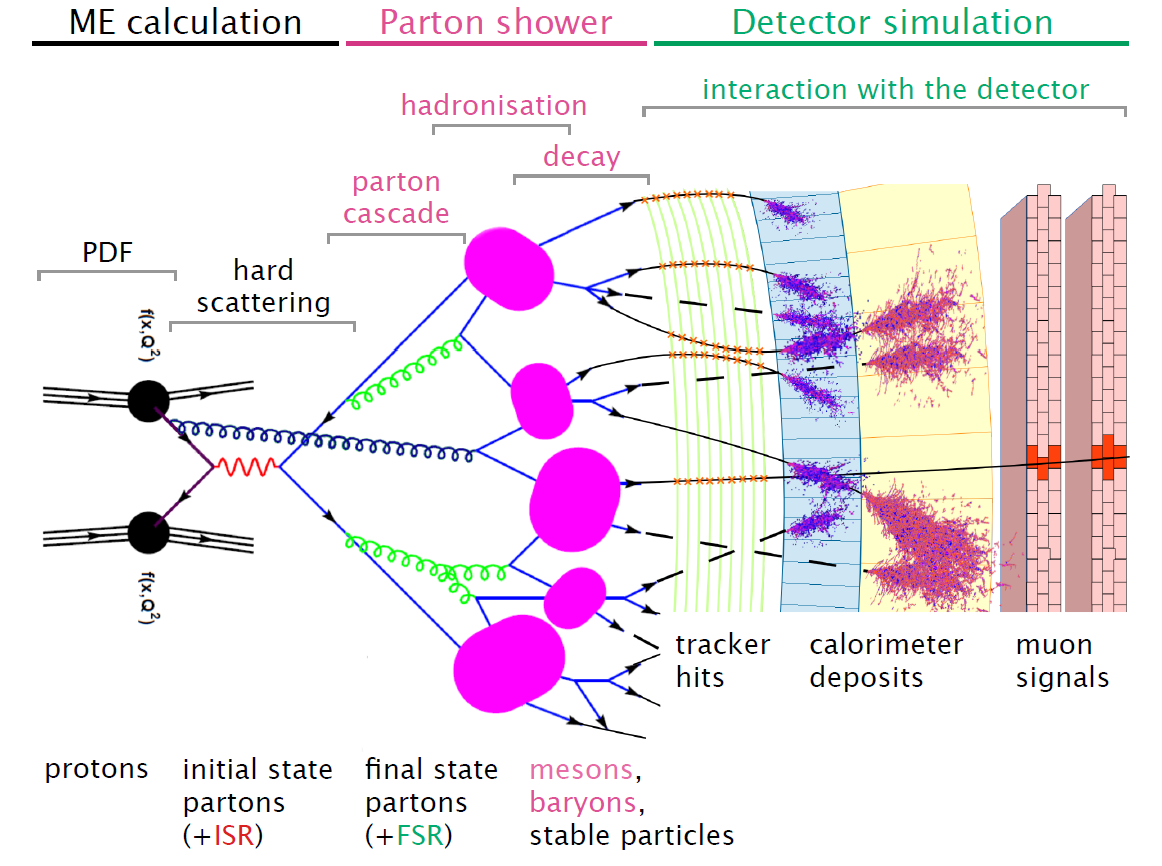
\includegraphics[width=\columnwidth]{../ThesisImages/Simulation/MCFlow.png}
	\caption[A pictoral view of the different steps for the creation of a MC event.]{A pictoral view of the different steps for the creation of a MC event. \cite{MaxThesis} 
	}
	\label{fig:SimMCFlow}
\end{figure}

\subsection{ Matrix Element Calculation and Parton Distribution Functions}

Particle interactions at LHC energies do not involve the entire proton.  The consituent partons that create the proton (the two up quarks, down quark, and the sea of gluons) are what interact in any given event.  The gluons create many virtual quark-antiquark pairs which can itneract as well.  The valence quarks, the ups and down that make up the proton, are the major portion of interacting partons at low energies, mainly inelastic interactions.  At LHC energies deep inelastic scattering is possible and the sea quarks play a more dominant role.  Proton structure is described by a Parton Distribution Function (PDF) which gives the probability of of finding any parton with a particular momentum fraction and is shown in Figure \ref{fig:PDF}.

\begin{figure}[h!]
	\centering
	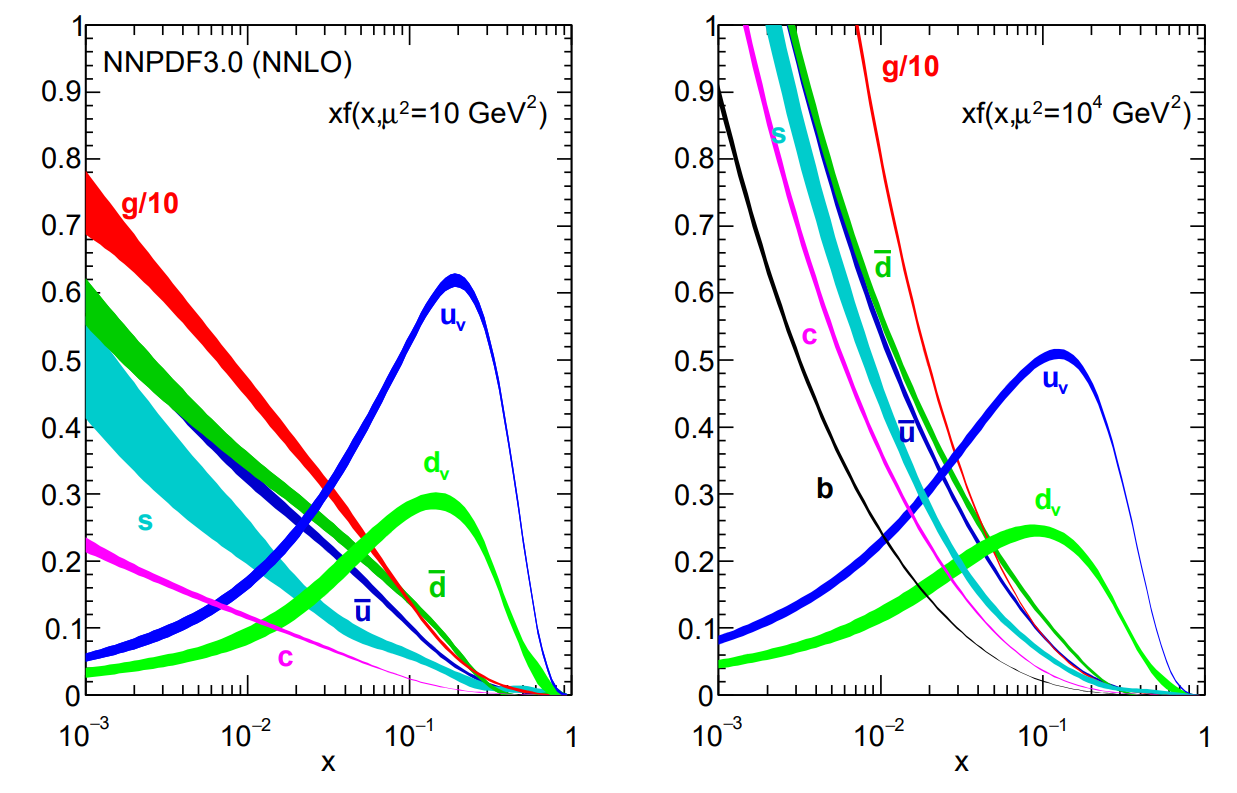
\includegraphics[width=\columnwidth]{../ThesisImages/Simulation/PDF.png}
	\caption[The bands are the momentum fraction, $x$, times the unpolarized parton distribution function obtained in NNLO NNPDF3.0 global analysis at scales $\mu^2= 10$ GeV and $\mu^2 = 100 \text{ GeV}^2$]{The bands are the momentum fraction, $x$, times the unpolarized parton distribution function obtained in NNLO NNPDF3.0 global analysis at scales $\mu^2= 10 \text{ GeV}^2$ and $\mu^2 = 100 \text{ GeV}^2$ \cite{PDG2018} 
	}
	\label{fig:PDF}
\end{figure}
The PDFs and hard scattering processes are included in the calulation of the Matrix Elements (ME) of any interaction.  Hard scattering processes can be descibed by Feynman diagrams, a representation of their amplitudes.  Combining the PDFs and hard scattering amplitudes gives the probability of a particular interaction occuring.  Calculation of the MEs is the first stage of simulation and is done to a specified order in perturbation theory: leading order (LO), next-to-leading order (NLO), etc.  Higher order calculations lead to more accurate predictions but grow in complexity exponentially making them hard to calculate both theoretically and computationally.  This is what often restricts how accurate a process can be simulated.  

\subsection{Parton Shower Calculation}
The next stage of simulating an event is the parton shower.  These parton shower calculations deal with the quantum chromodynamic processes.  In any interaction the particles that carry color can spontaneously emit gluons which can go on to create more gluons or quark-antiquark pairs.  Depending on when this happens in the hard scattering process it is called initial state radiation (ISR) or final state radiation (FSR).   The hard scattering partons as well as any additional radiated particles are used as inputs to parton shower calculations which determine how the quarks and gluons proceed through to the final state particles seen in the detector.  This includes calculation of hadronization processes and futher decay processes into the final state particles.

\subsection{Detector Simulation}
The final stage of creating a MC event is the detector simulation.  The information from the event generators are processed using \textsc{geant4} \cite{Geant4} and a detailed model of the ATLAS detector.  \textsc{geant4} simulates how various particles propagate through and interact with the material properties of the detector and where they leave energy which would then be measured by the ATLAS detector in an actual event.  The result of this MC event construction flow is a collection of simulated data that is similar in structure to actual data collected using the ATLAS experiment.  The energy deposits in both MC and real data are then reconstucted using the same software and physics objects are reconstructed.  For MC this allows for comparison between the physics object reconstruction and the truth record, or the types of particles fed into the detector simulation.

\subsection{Monte Carlo Generators Used for LHC Physics}

A variety of different MC generators are used in the creation of simulated events.  Different generators can sepecializing in simulating different physics processes and handle various precision (eg., LO vs. NLO). The MC generators used in this search are summarized in this section.

\textsc{MadGraph} aMC@NLO \cite{MadGraph}: An amplitude and event generator at LO and NLO for hard processes.  Extendable to various models including effective field theory (EFT) models used in BSM searches.  This generator is used to create the signal events searched for in this dissertation: discussed in Section \ref{Sec:MG5Sig}. 

\textsc{powheg} \cite{Powheg1,Powheg2}: \textbf{Po}sitive \textbf{W}eight \textbf{H}ardest \textbf{E}mission \textbf{G}enerator is an NLO event generator that can be interfaced with other generators (i.e. \textsc{pythia}) for showering.

\textsc{pythia} \cite{Pythia8}: A generator used most often for QCD final state hard processes and showering.  It is commonly interfaced with other generators for showering within the ATLAS detector.
\textsc{sherpa} \cite{Sherpa11,Sherpa22}: A multi-parton LO generator with an emphasis on merging ME and Parton Showering.

These generators are commonly interfaced, usually with \textsc{pythia} for showering, and this is possible due to a common file format developed at the Les Houches Accords \cite{Alwall:2006yp}.  This allows a specialty generator to be created and used to generate hard processes and then simulate the rest of the event with common showering generators that might lack the ability to simulate the process in question.

\section{Object Reconstruction}

After the events are simulated, or collected in case of real data, all there is is a collection of energy deposits within the detector.  These energy deposits must be transformed into meaningful physics objects through reconstruction.  Reconstruction is typically done in two major parts using the specialized detectors covered in Chapter \ref{ch:LHCDetector}.  The Inner Detector and Muon System turn patterns of hits within the tracking detectors into tracks that have direction and momentum information.  The calorimeter system transforms the energy deposits within the calorimeters into calibrated energy deposits with a particular position.  These tracks and calorimeter deposits are used to create physics objects (electrons, muons, etc.) by using particle identification techniques to reconstruct the underlying physics event.  For the analysis presented in this dissertation the final state signal particles that need to be reconstructed are one lepton (an electron or a muon), one photon, two quarks (one light flavor and on b quark), and one neutrino (missing transverse energy as it is the only particle that does not interact with the detector).  Each of these particles has a particular signature in the subdetectors of the ATLAS detector, shown in Figure \ref{fig:ATLASInteractions}.

\begin{figure}[h]
	\centering
	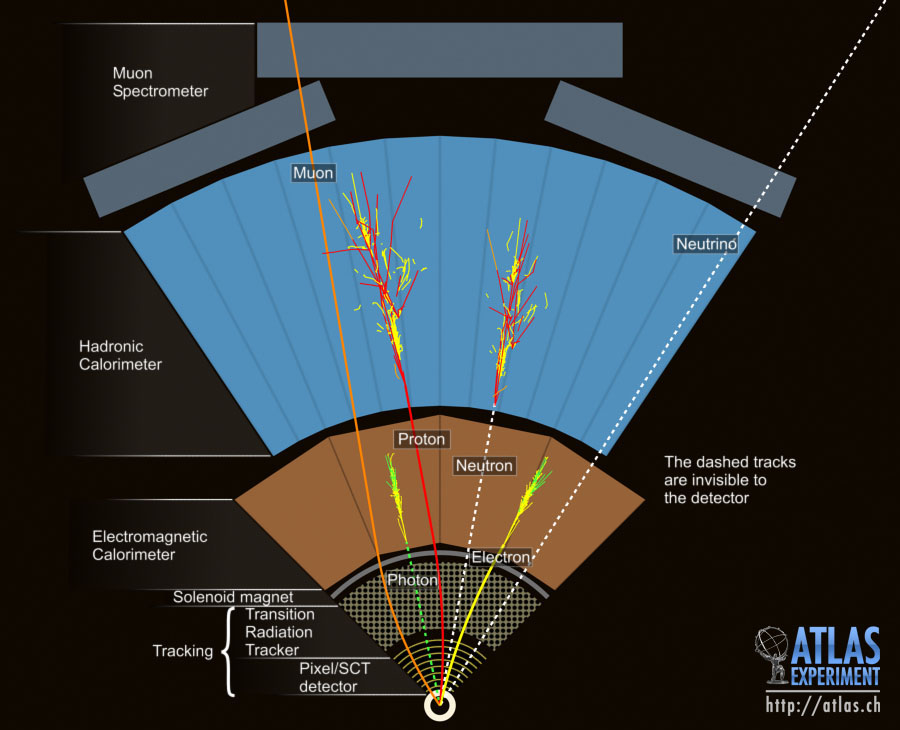
\includegraphics[width=\columnwidth]{../ThesisImages/Simulation/ParticleInteractions.jpg}
	\caption[Cross section of a simulated ATLAS detector showing how various particles interact with ATLAS subsystems.]{Cross section of a simulated ATLAS detector showing how various particles interact with ATLAS subsystems.  Solid lines indicate interactions while dashed lines indicate that no interactions typically occur in that section of the detector. \cite{ParticleInteractions} 
	}
	\label{fig:ATLASInteractions}
\end{figure}


\subsection{Electrons}
Electrons interacting with the ATLAS detector leave a track in the Inner Detector as well as a cluster of energy in the electromagnetic calorimeter.  The track and cluster are required to be matched together to be identified as an electron candidate\cite{ElectronID}.  As electrons move through the detector they create electromagnetic showers through bremsstrahlung which can produce electron-positron pairs.  The process continues as the particles continue to give energy to the detector.  This collection of electrons, positrons, and photons creates a signature energy cluster in the calorimeter.  

Electron identification algorithms are applied to the electron candidates to separate prompt and isolated electron candidates from electrons that come from backgrounds such as converted photons and misidentified jets.  The electron idenification algorithms use a sliding window ( $3\times5$ in $\eta \times \phi$) in the high granularity section of the LAr electromagnetic calorimeter to search for electron cluster ``seeds'' greater than 2.5 GeV.  Clusters are created around these seeds to form the electromagnetic shower and remove possible duplicate electron signals by containing them within the cluster.  Further pattern recognition for the track fitting allows even larger amounts of energy into the shower to account for bremsstrahlung in the shower shape.  Tracks and clusters are then matched to give electron candidates.  

Electrons coming from background jets or photon conversion are called non-prompt as they do not originate from a signal object.  In order to reject these electrons other discriminating variables are used in addition to the track-cluster matching.  Variables such as the energy leakage into the hadronic calorimeter, how the shower developed throughout the electromagnetic calorimeter, and the amount of radiation measured in the TRT.  Three electron identification working points are used: Loose, Medium, and Tight.  Each of these operating points have their own level of background rejection and signal efficiency.  Working points with higher background rejection are a subset of those with lower background rejection.

Isolation variables are another useful tool in the identification of signal electrons from converted photons produced in hadron decays and light hadron misidentification.  These variables are defined by a cone size around the electron candidate and are the sum of the transverse variable (momentum or energy) of all of the tracks within the cone, $p_{T}^{\text{varcone0.2}}$ with a cone of $\Delta R =0.2$ (or 10 GeV/$E_T$, for high energy electrons) and $E_{T, Topo}^{\text{varcone0.4}}$ with a cone definied in a similar manner.  

Since the LAr calorimeter is a sampling calorimeter the energy deposits must be calibrated and scaled such that the true electron energy is read out not just the small amount of energy deposited into the active layers as discussed in Section \ref{sec:EMHCal}.  The energy scale is calibrated to be uniform throughout the detector.  Any residual differences between data and simulation are corrected.  The calibration strategy was developed for optimal preformance in LHC Run 1\cite{ElectronCalib1} and updated for the conditions of LHC Run 2\cite{ElectronCalib2}.

\subsection{Muons}
Muons behave differently than other particles as they go through the detector.  They act as minimum-ionizing-particles (MIPs) throughout the calorimeter.  The Muon Spectrometer (MS), Section \ref{sec:MuCal}, specializes in precision measurements of muons.  The Inner Detector (ID) plays a pivotal role in the identification of muons as it offers an independent measure of the muon characteristics.  Reconstructing muons use a specific set of variables as well\cite{MuonID}.  These variables include \textit{ q/p significance}: the difference in the ratio of track charge and momentum measured with the ID and MS, $\rho'$: the difference between the transverse momenta measured with the ID and MS, and the $\chi^2$ of the combined track fit using tracks from both the ID and MS.

Muons are separated out into four separate types depending on their interactions with the various subdetectors.  The best muon candidates are combined muons which use hits in the MS to trace back to a track in the ID to reconstruct the entire muon track.  Segment-tagged muons are muon candidates that leave a track in the ID but only a segment in the MS instead of a full track, this can occur because of the muon having low $p_T$ or crossing through a region of the MS with reduced acceptance.  Extrapolated muons require only tracks in the MS and are used in regions of $\eta, \phi$ phase space that the ID does not cover.  Calorimeter-tagged muons are muons identified by MIPs in the calorimeters and are used to find muons that cross the ID and MS in regions where cabling might prevent particle detection.

Muons also have their own set of isolation criteria which is track-based $p_{T}^{\text{varcone0.3}}$, with a cone of $\Delta \text{R} = \text{min}(0.3,10\text{ GeV}/p_T)$.  Similar to electrons various working points are available for at the analysis level for muons.  These working points are named similarly: Loose, Medium, Tight, and High-$p_T$ in order of background rejection.  

High $p_T$ jets that punch through the hadronic calorimeter can leave tracks in the MS which could be identified as muons.  These would be identified as a bad or a fake muon because of the high hit multiplicities they leave in the MS as opposed to a single track left by a muon as it is a MIP.  Another source of bad muons is a mis-measured ID track that gets incorrectly matched to segments in the MS.  Fake muons are a source of fake missing transverse energy, $ \slashed{E}_T$

\subsection{Photons}
Photons behave very similarly to electrons in the calorimeter in that they produce an electromagnetic shower in the calorimeter.  However, they are neutrally charged particles meaning that they should not leave a track in the ID as they do not bend and produce bremsstrahlung photons travelling through the magnetic field.  Prompt photons pair-produce electrons in the tracker but this process can be picked out as the associated cluster in the electromagnetic calorimeter is matched to two opposite charged tracks.  This process is called a converted photon.  Unconverted photons have no matching tracks associated to an electromagnetic cluster.    

\begin{center}
\begin{table}
\noindent\makebox[\textwidth]{%
\small
{\renewcommand{\arraystretch}{1.6}
\begin{tabularx}{1.25 \textwidth}{ l X lll }
\hhline{=====}
Category 	& Description  & Name  & \textit{loose}  & \textit{tight} \\ \hline
Acceptance 	& $|\eta|<2.37$, with $1.37 \leq |\eta|<1.52$ excluded  & -  &  \checkmark  & \checkmark \\
Hadronic Leakage & Ratio of $E_T$ in the first sampling layer of the hadronic calorimeter to $E_T$ of the EM cluster (used over the range $0.8<|\eta|$ or $|\eta|>1.52$) & $R_{\text{had}_1}$  &  \checkmark  &  \checkmark \\
		&  Ratio of $E_T$ in the hadronic calorimeter to $E_T$ of the EM cluster (used over the range $0.8<|\eta|<1.37$) & $R_{\text{had}}$  &   \checkmark &  \checkmark \\
EM Middle Layer & Ratio of the energy in $3\times 7$ $\eta \times \phi$ cells over the energy in $7\times 7$ cells centered around the photon cluster position & $R_{\eta}$ &   \checkmark &  \checkmark \\
		 & Lateral shower width, $\sqrt{(\Sigma E_{i} \eta_{i}^2 )/(\Sigma E_i )-((\Sigma E_i \eta_i )/(\Sigma E_i))^2}$, where $E_i$ is the energy and $\eta_i$ is the pseudorapidity of cell i and the sum is calculated within a window of $3\times 5$ cells & $\omega_{\eta_2}$ &  \checkmark &   \checkmark\\
		 & Ratio of the energy in $3 \times 2$ $\eta \times \phi$ strips, over the energy of $3\times 6$ cells centered around the photon cluster position  & $R_\phi$ &  &  \checkmark \\
EM Strip Layer & Lateral shower width, $\sqrt{(\Sigma E_i (i-i_\text{max})^2)/(\Sigma E_i)}$, where i runs over all strips in a window of $3 \times 2$ $\eta \times \phi$ strips, and $i_{\text{max}}$ is the index of the highest-energy strip calculated from three strips aroudn the strip with maximum energy deposit & $\omega_{s\text{ 3}}$  &  & \checkmark \\
		 & Total lateral shower width  $\sqrt{(\Sigma E_i (i-i_\text{max})^2)/(\Sigma E_i)}$, where i runs over all strips in a window of $20 \times 2$ $\eta \times \phi$ strips, and $i_{\text{max}}$ is the index of the highest-energy strip measured in the strip layer & $\omega_{s\text{ tot}}$  &  &  \checkmark \\
		 & Energy outside the core of the three central strips but within seven strips divided by energy within the three central strips  & $f_\text{side}$ &  &  \checkmark  \\
		 & Difference between the energy associated with the second maximum in the strip layer and the energy reconstructed in the strip with the minimum value found between the first and second maxima & $\Delta E_s$ &  &   \checkmark \\
		 & Ratio of the enrgy difference between the maximum energy deposit and the energy deposit in the secondary maximum in the cluster to the sum of these energies & $E_\text{ratio}$ &  &  \checkmark \\
		 & Ratio of the energy in the first layer to the total energy of the EM cluster & $f_1$ &  &  \checkmark \\
\hhline{=====}
\end{tabularx}
\normalsize
}}
\caption[Photon identification variables used for \textit{loose} and \textit{tight} photon identification]{Photon identification variables used for \textit{loose} and \textit{tight} photon identification, taken from \cite{PhotonID}}
\label{tab:PhotonVars}

\end{table}
\end{center}

Prompt photons produce narrower energy deposits in the electromagnetic calorimeter and have smaller leakage into the hadronic calorimeter compared to background photons.  The energy contained within narrow structure in $\eta \times \phi$ strips compared to the energy containd in a larger section can help pickout prompt from non-prompt photons \cite{PhotonID}.  Cuts on this and the other variables listed in Table \ref{tab:PhotonVars} are tuned to reduce dependency of identification efficiency on the pileup conditions of Run 2.


\subsection{Jets}

Contrasting with electromagnetic showers produced by electrons and photons, hadronic showers from through QCD processs.  Quarks very quickly undergo showering by emitting gluons which further produce quark-antiquark pairs in analogy to the photons and pair produced electron-positron pairs of electromagnetic showers.   When quarks have enough energy they hadronize by producing bound states of particles.  These particles are typically pions or mesons that are measured by the ATLAS detector.  The top quark is the only quark that decays before hadronization because it decays so fast ($5\times10^{-25}$ s).  The spray of hadrons coming from a quark from the initial interaction is called a jet and is a collection of detector objects that are traced back and assigned to the quark(s) in the final state of the interaction.  The algorithms that do this are called jet-finding algorithms and pictoral representations of the same event reconstructed with four various algorithms is shown in Figure \ref{fig:VarJetAlgs}.

%Ben\cite{CambridgeAachen}
%Ben\cite{JetCleaning}
\begin{figure}[h!]
	\centering
	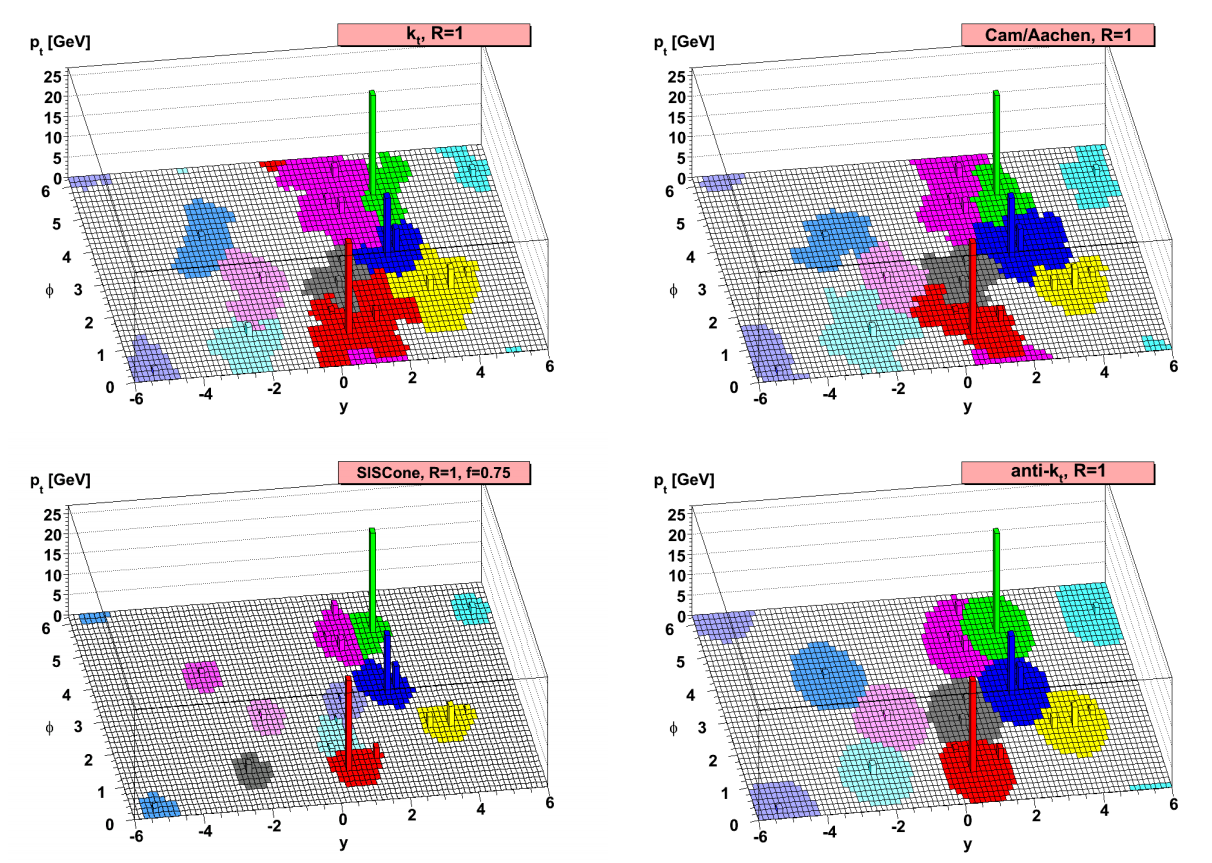
\includegraphics[width=\columnwidth]{../ThesisImages/Simulation/VarJetAlgs.png}
	\caption[A sample parton-level event with many random soft jet objects, clustered with four different jets algorithms, illustrating the areas of the resulting hard jets. For kt and Cambridge/Aachen the detailed shapes are in part determined by the specific set of ghosts used, and change when the ghosts are modified]{A sample parton-level event with many random soft jet objects, clustered with four different jets algorithms, illustrating the areas of the resulting hard jets. For kt and Cambridge/Aachen the detailed shapes are in part determined by the specific set of ghosts used, and change when the ghosts are modified \cite{antikt} 
	}
	\label{fig:VarJetAlgs}
\end{figure}

The jets used in this analysis use the anti-$k_T$ algorithm \cite{antikt} with a radius parameter $R=0.4$.  Jets are not physical objects but collections of them so how they are defined can change the physics objects that are eventually analyzed.  The anti-$k_T$ algorithm is preferred because it is infrared and collinear safe.  Infrared safe jet algorithms do not merge two jets with a soft emission between them.  Adding or removing a soft term between two jets should not change what objects are called jets.  Collinear safe jet algorithms do not change the jet collection if you split or merge the high transverse momentum particles.  Another added benefit of the anti-$k_T$ jet finding algorithm is that it gives roughly circular jet objects which simplifies calculating the energy density making calibrating the physics object simple.

The anti=$k_T$ algorithm calculates the distance between an object $i$ and all possible jet objects $j$ ($d_{ij}$) and the beam ($d_{iB}$)
\[ d_{ij} = \text{min}(k_{ti}^{2p},k_{tj}^{2p})\frac{\Delta^2_{ij}}{R},\qquad 
d_{iB} = k_{ti}^{2p} \] 
where $k_{ti}$ is the transverse momentum, $\Delta$ is the distance between the objects, and $p=-1$.  This is a general form for the type of algorithm, the inclusive $k_T$ algorithm has a p value of 1 and the inclusive Cambridge/Aachen algorithm has a p value of 0 \cite{CambridgeAachen}.  The algorithm then follows that if $d_{ij}$ is smaller than$d_{iB}$ then objects $i$ and $j$ are merged, otherwise $i$ is labeled as a jet and removed from the list of entries of possible jet objects.  This is repeated for all entries in the list of possible jet objects.

Jet cleaning is also applied to remove events with jets built from known noisy parts of the calorimeter due to particular calorimeter cells or non-collision background in those areas \cite{JetCleaning}.  To reduce selecting jets that originate from pileup interactions another requirement on the jet object is made on the jet vertex tagger \cite{JetJVT, JetCleanTwiki} as follows:
\begin{enumerate}
\item For jets with $20 \mathrm{ GeV } < p_{T} < 60 \mathrm{ GeV }$ and $|\eta| < 2.4$: if any jet is bad AND that jet is not marked as pileup by JVT, then reject the event
\item For jets with $20 \mathrm{ GeV } < p_{T} < 60 \mathrm{ GeV }$ and $|\eta| \geq 2.4$: if any jet is bad, then reject the event
\item For jets with $p_{T} \geq 60 \mathrm{ GeV }$: if any jet is bad, then reject the event
\end{enumerate}
\subsubsection{B-Jets}


\begin{figure}[h!]
	\centering
	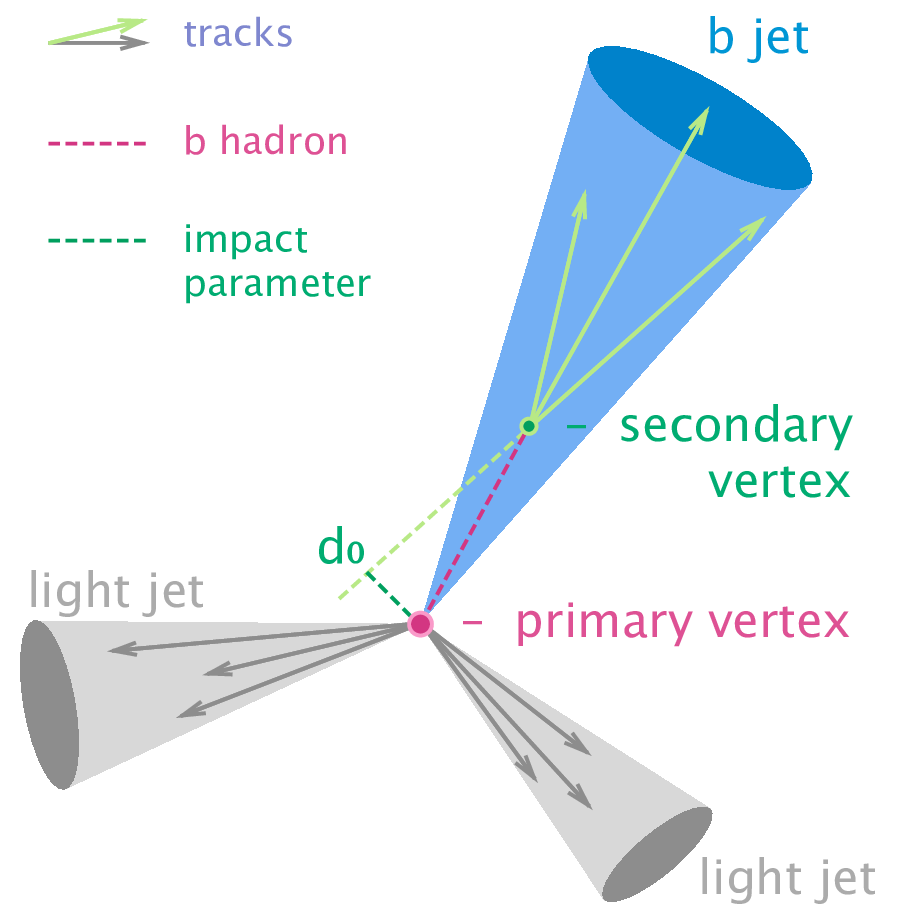
\includegraphics[width=.5\columnwidth]{../ThesisImages/Simulation/B-tagging_diagram.png}
	\caption[C]{\cite{Takubo:2017wvt} 
	}
	\label{fig:BTagVars}
\end{figure}

\begin{figure}[h!]
	\centering
	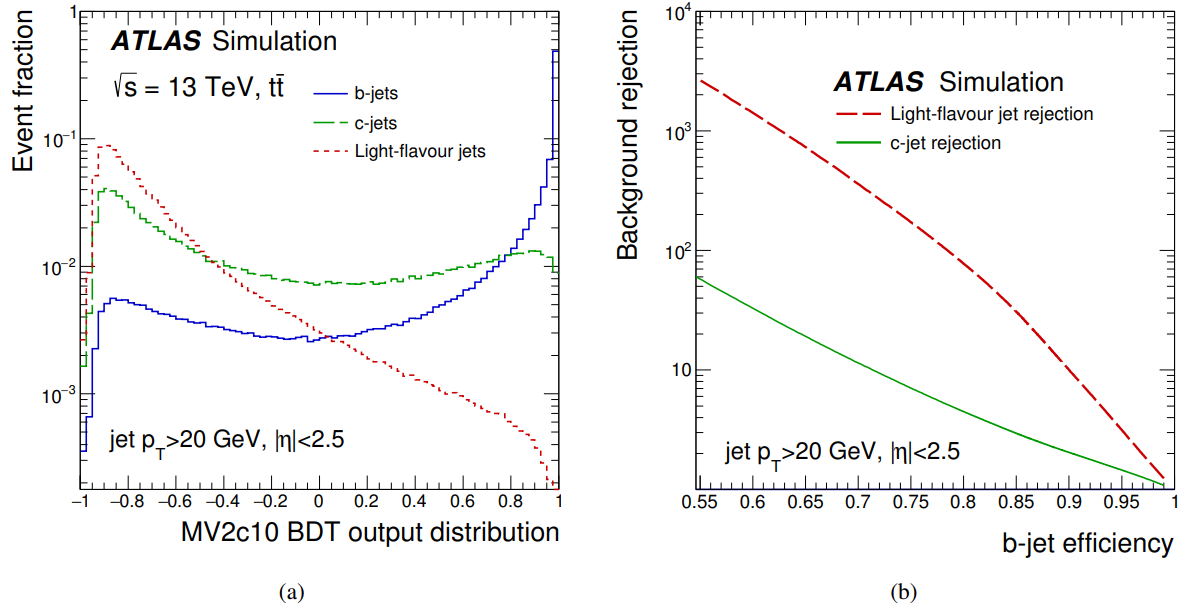
\includegraphics[width=\columnwidth]{../ThesisImages/Simulation/BTagMV2c10andRejVsEff.png}
	\caption[C]{\cite{Takubo:2017wvt} 
	}
	\label{fig:BTag}
\end{figure}


%\cite{Takubo:2017wvt}%IBL Preformance
\label{sec:bjetReco}

\subsection{Missing Transverse Energy}
\cite{METreco}

\section{Creation of Flavor Changing Neutral Current Signal Events}
\label{Sec:MG5Sig}
\subsection{MadGraph5 amc@NLO}
Comparison of kinematics between standard ttbar events

- param card in appendix

ATLAS Production of these events

TopQ1 Slimming/Skimming








%
%%%%%%%%%%%%%%%%%%%%%%%%%%%%%%%%%%%%%%%%%%%%%%%
%%%%%%%%%%%%                                                                                                   %%%%%%%% 
%%%%%%%%%%%%                           BEN                                                                  %%%%%%%% 
%%%%%%%%%%%%                                                                                                   %%%%%%%% 
%%%%%%%%%%%%%%%%%%%%%%%%%%%%%%%%%%%%%%%%%%%%%%%
%
%
%\chapter{The Strong Force and Jets}
%\label{ch:Jets}
%
%The cross-section for the collision of two hadrons can be written as
%\begin{equation}
%d\sigma_{AB\rightarrow J+X} = \sum_{a,b}^{}\int dx_a dx_b f_{a/A}(x_a, \mu_F^2) f_{b/B}(x_b, \mu_F^2) \times d\hat{\sigma}_{ab\rightarrow J+X} (\alpha_s(\mu^2_R),Q^2)
%\end{equation}
%where $A$ and $B$ are the incoming hadrons (in the case of the LHC, protons), $J+X$ are an observable plus any other particle, such as two jets, or a jet plus some invisible particle, $a$ and $b$ are the types of partons (the six quark flavors and the gluon), $d\hat{\sigma}_{ab\rightarrow X} (\alpha_s(\mu^2_R),\mu^2)$ is the cross-section for the collision of the two partons $a$ and $b$ to produce $X$, which can be calculated directly from theory and depends on the the scale of the interaction, $\mu$, and strong QCD coupling, $\alpha_s$, measured at renormalization scale $\mu^2_R$.  This formula is approximate and has corrections of surpressed by a factor of 1~GeV/$Q$.  For the energies probed in this analysis, with jets on the order of 1~TeV, these corrections are very small.
%
%The renormalization scale is used to absorb the ultraviolet divergences which come from the higher-order diagrams of the process, imposing a cutoff on the energy in exchange for making $\alpha_s$ depend on this scale.\cite{StrongCoupling}  This is the origin of the running coupling of the strong interaction, where the strength of the coupling decreases as the energy of the process increases.  Similarly, the parton distribution functions discussed in the next section depend on the choice of factorization scale.  
%
%While the choice of scale is arbitrary and should not have an effect on the cross-section, this is only true if one is able to expand out to infinite accuracy, as $\hat{\sigma}$ has an expansion in powers of $\alpha_s$.  With a good choice in scale, good accuracy to the full expansion can be obtained with only a few terms in the series.   With the choice of renormalization and factorization scales close to the scale of the given process such that $\mu^2_R = \mu_F^2 \simeq Q^2$, the cross-section can be characterized by only the energy scale of the interaction and is well described by the expansion.  This choice of scales is used for the remainder of this chapter.
%
%The final factors, $f_{a/A}(x_a, Q^2)$, are the parton distribution functions, or PDFs.  The PDFs represent the probability density for a parton of type $a$ to carry a fraction $x_a$ of the total momentum of the hadron.  The total cross section for the process is then the sum over all of the types of partons from the two incoming hadrons.
%
%
%
%\section{Parton Distribution Functions}
%
%Since the proton is a composite particle, its overall momentum is equivalent to the sum of the momenta of its constituents.  Given the large momenta of accelerated protons in the LHC for Run 2, this is equivalent to saying that the total energy of the proton (6.5\,TeV for Run 2) is divided up between the partons that comprise the proton.
%
%PDFs can not be calculated from theory but instead must be taken directly from data, much of which comes from deep inelastic scattering experiments from electron-proton colliders, in addition to Drell-Yan and inclusive jet production measurements from proton-proton colliders, including results from Run 1 of the LHC.  Once the PDF at a given energy transfer $Q$ is known, the PDF can be evolved to other energies using the Dokshitzer-Gribov-Lipatov-Altarelli-Parisi~(DGLAP) equations.\cite{DGLAP1,DGLAP2,DGLAP3}  Examples of the proton PDF at two different energy scales are shown in Figure~\ref{fig:CT14PDFs}.  
%
%While one would naively expect the momentum to be roughly split between the two up quarks and one down quark, this is not the case.  Rather, a sizeable portion of the momentum is carried by gluons which constantly radiate from and are reabsorbed by the valence quarks.  These gluons can also fluctuate into quark-antiquark pairs, referred to as $sea~quarks$.  At higher $Q$, shorter distance scales are probed, meaning larger fluctuations are accessible, and thus larger amounts of momentum are carried by the gluons and sea quarks rather than just by the valence quarks.
%
%\begin{figure}[h!]
%	\centering
%	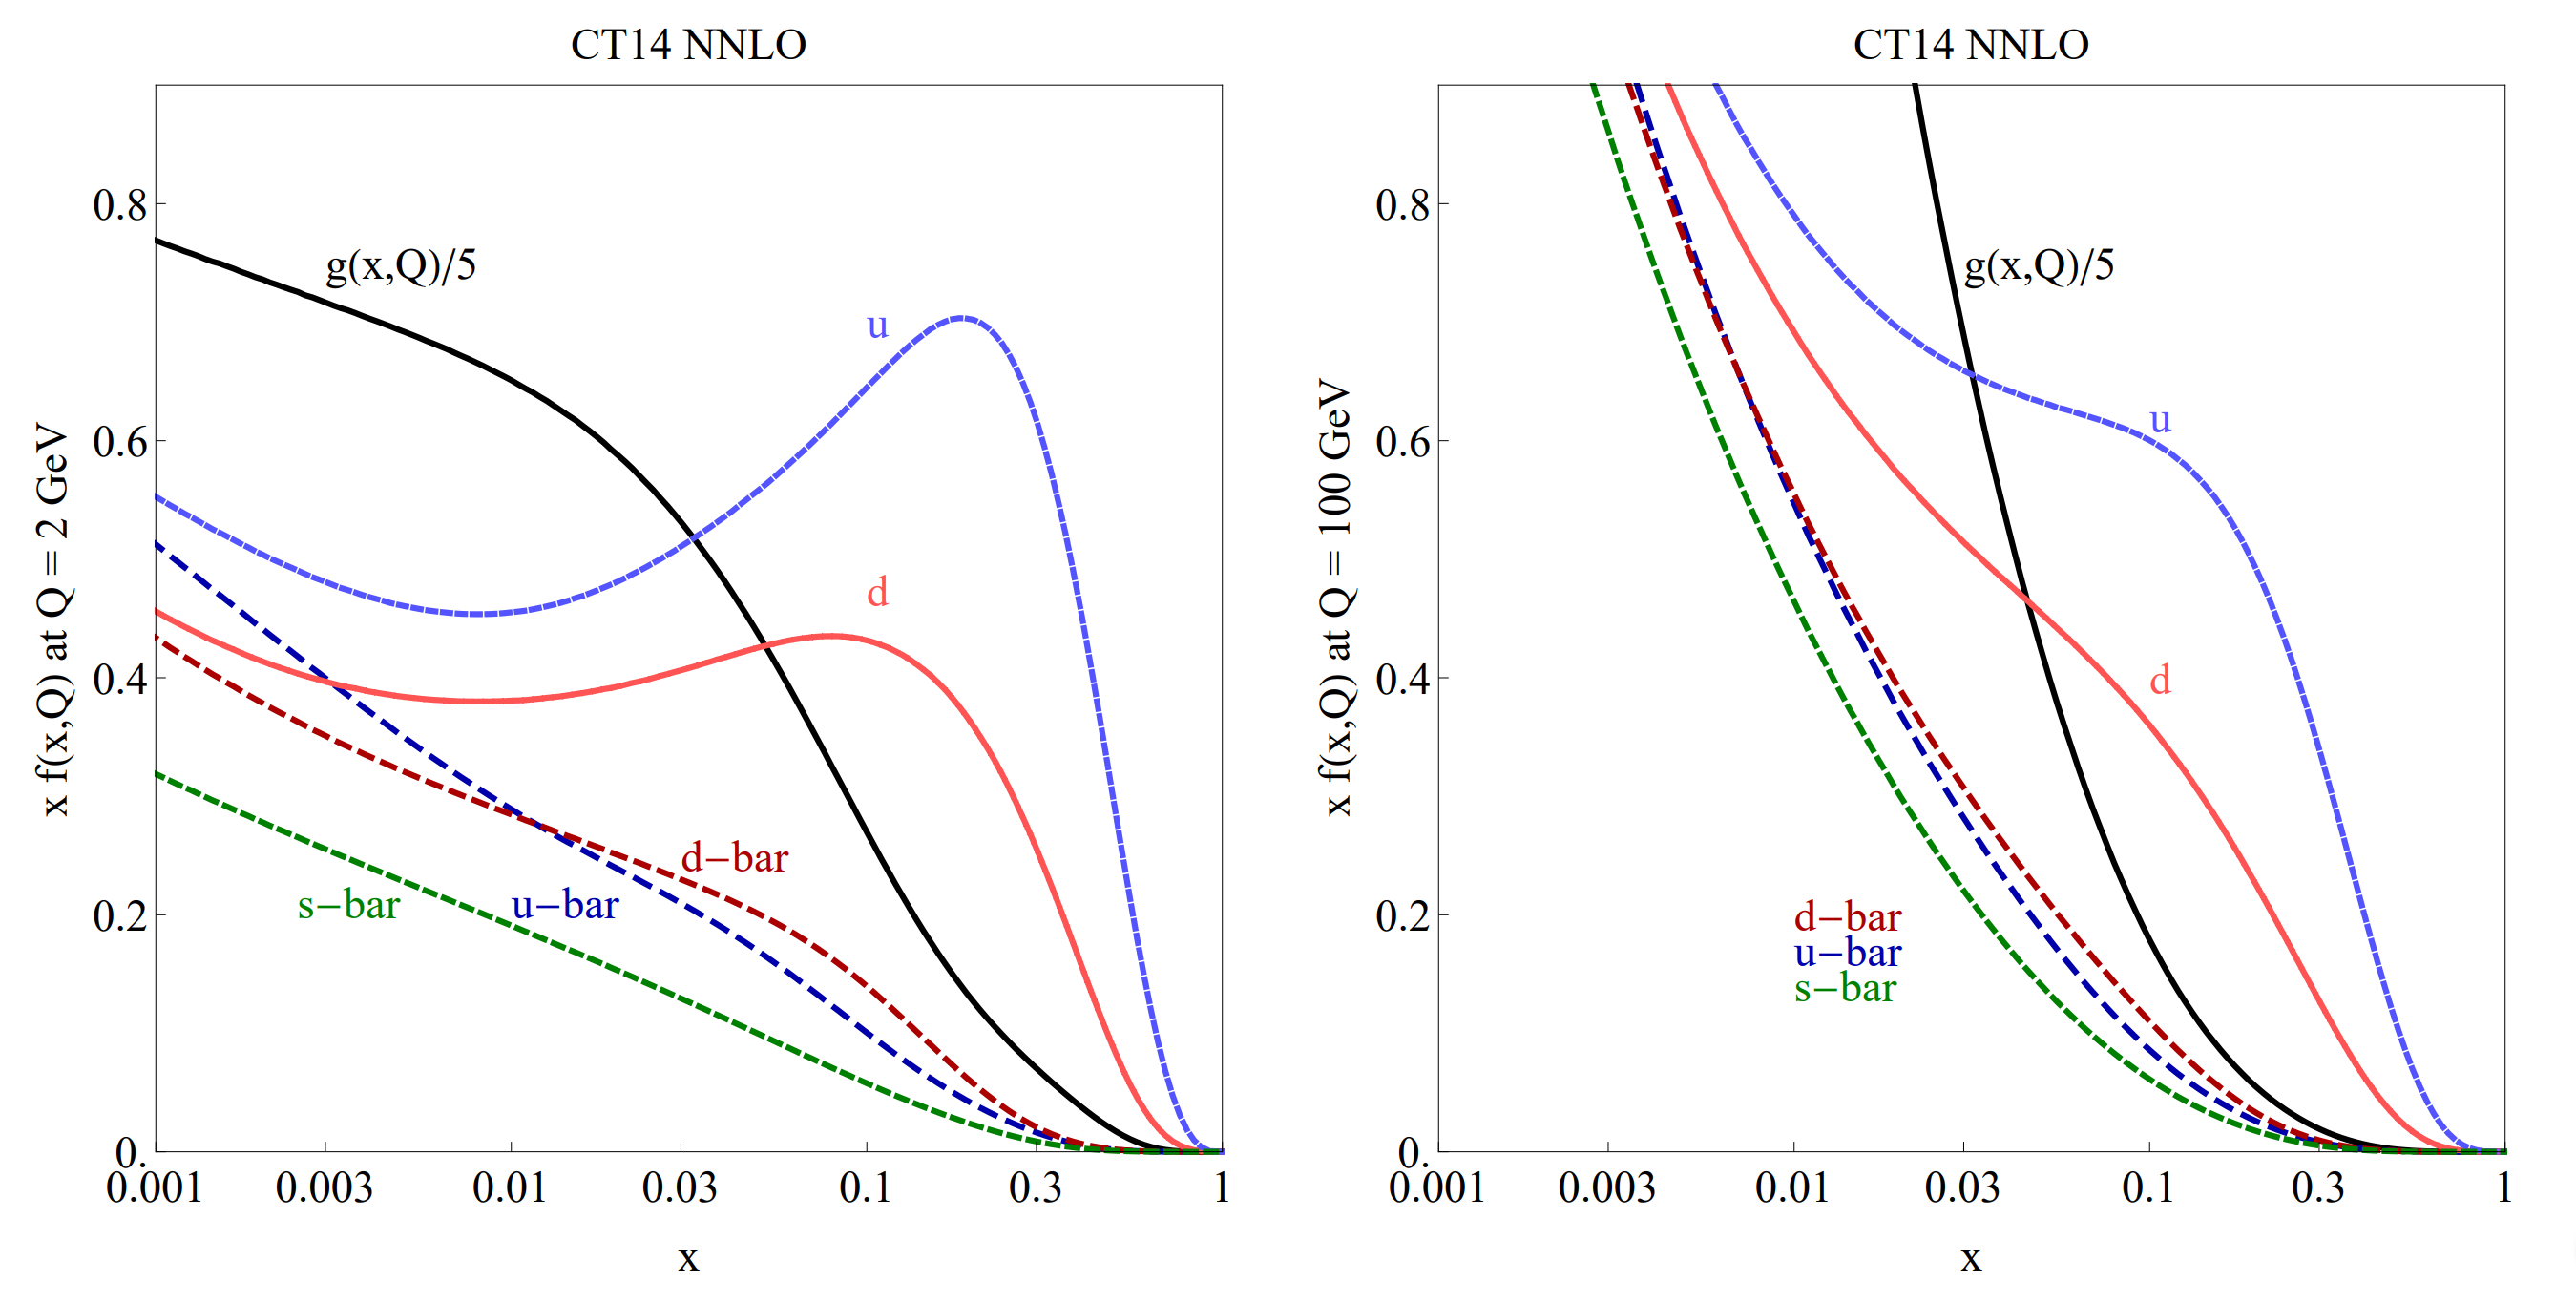
\includegraphics[width=\columnwidth]{figures/Jets/CT14PDFs.png}
%	\caption{The measurement of parton distribution functions (PDFs) from the CTEQ collaboration. PDFs are shown at Q = 2\,GeV and Q = 100\,GeV for $u, \bar{u}, d, \bar{d}, s = \bar{s}$, and $g$.  The full results can be seen in Ref.~\cite{CT14PDF}.
%	}
%	\label{fig:CT14PDFs}
%\end{figure}
%
%The high-mass dijet search relies on interactions at high-$Q$ and partons at very high-$x$ in the PDF, where $x$ is the fraction of the total proton momentum carried by a given parton.  However, while the valence quarks are the most common at high-$x$, there are no quark-quark vertices in the standard model, only quark-antiquark and (anti)quark-gluon ones.  The t-channel quark-quark scattering is then the dominant background in a dijet search over s-channel processes from both Standard Model QCD and any possible new resonances.  Figure~\ref{fig:Feynman} shows a comparison of these two channels.  This background is suppressed in the analysis by imposing a maximum difference in rapidities between the two leading jets, as t-channel processes peak at very high rapidity near the beam line.  In the limit of massless quarks (a safe assumption given the energies probed by the high-mass dijet search), the Mandlestam variables can be written as:
%
%\begin{equation}
%\hat{s} = (p_1+p_2)^2 = \mjj^2
%\end{equation}
%\begin{equation}
%\hat{t} = -\frac{1}{2}\hat{s}(1-cos~\theta^*)
%\end{equation}
%where $\theta^*$ is the polar angle from the beam line to the outgoing parton in the center-of-mass frame, and \mjj~is the invariant mass of the dijet system.\cite{EllisQCD}  The matrix element for the $s$-channel process is proportional to $\hat{s}^{-1}$, while the $t$-channel process is proportional to $\hat{t}^{-1}$.  Thus, the $s$-channel production is independent of angle, while the $t$-channel mode peaks at angles close to the beam line and is minimized in the central region of the detector.
%
%\section{Anatomy of a Collision}
%
%While the Feynman diagrams for dijet production look simple, proton-proton collisions are extremely convoluted, as evidenced by Figure~\ref{fig:HadronEvent}.  In addition to the hard scatter and decays (in red), the event also contains many gluon emissions from the strongly charged particles (blue) as well as secondary interactions from the other proton constituents (purple).  These colored particles then group into colorless baryons and mesons, which in turn have their own decays (green).
%
%\begin{figure}[h!]
%	\centering
%	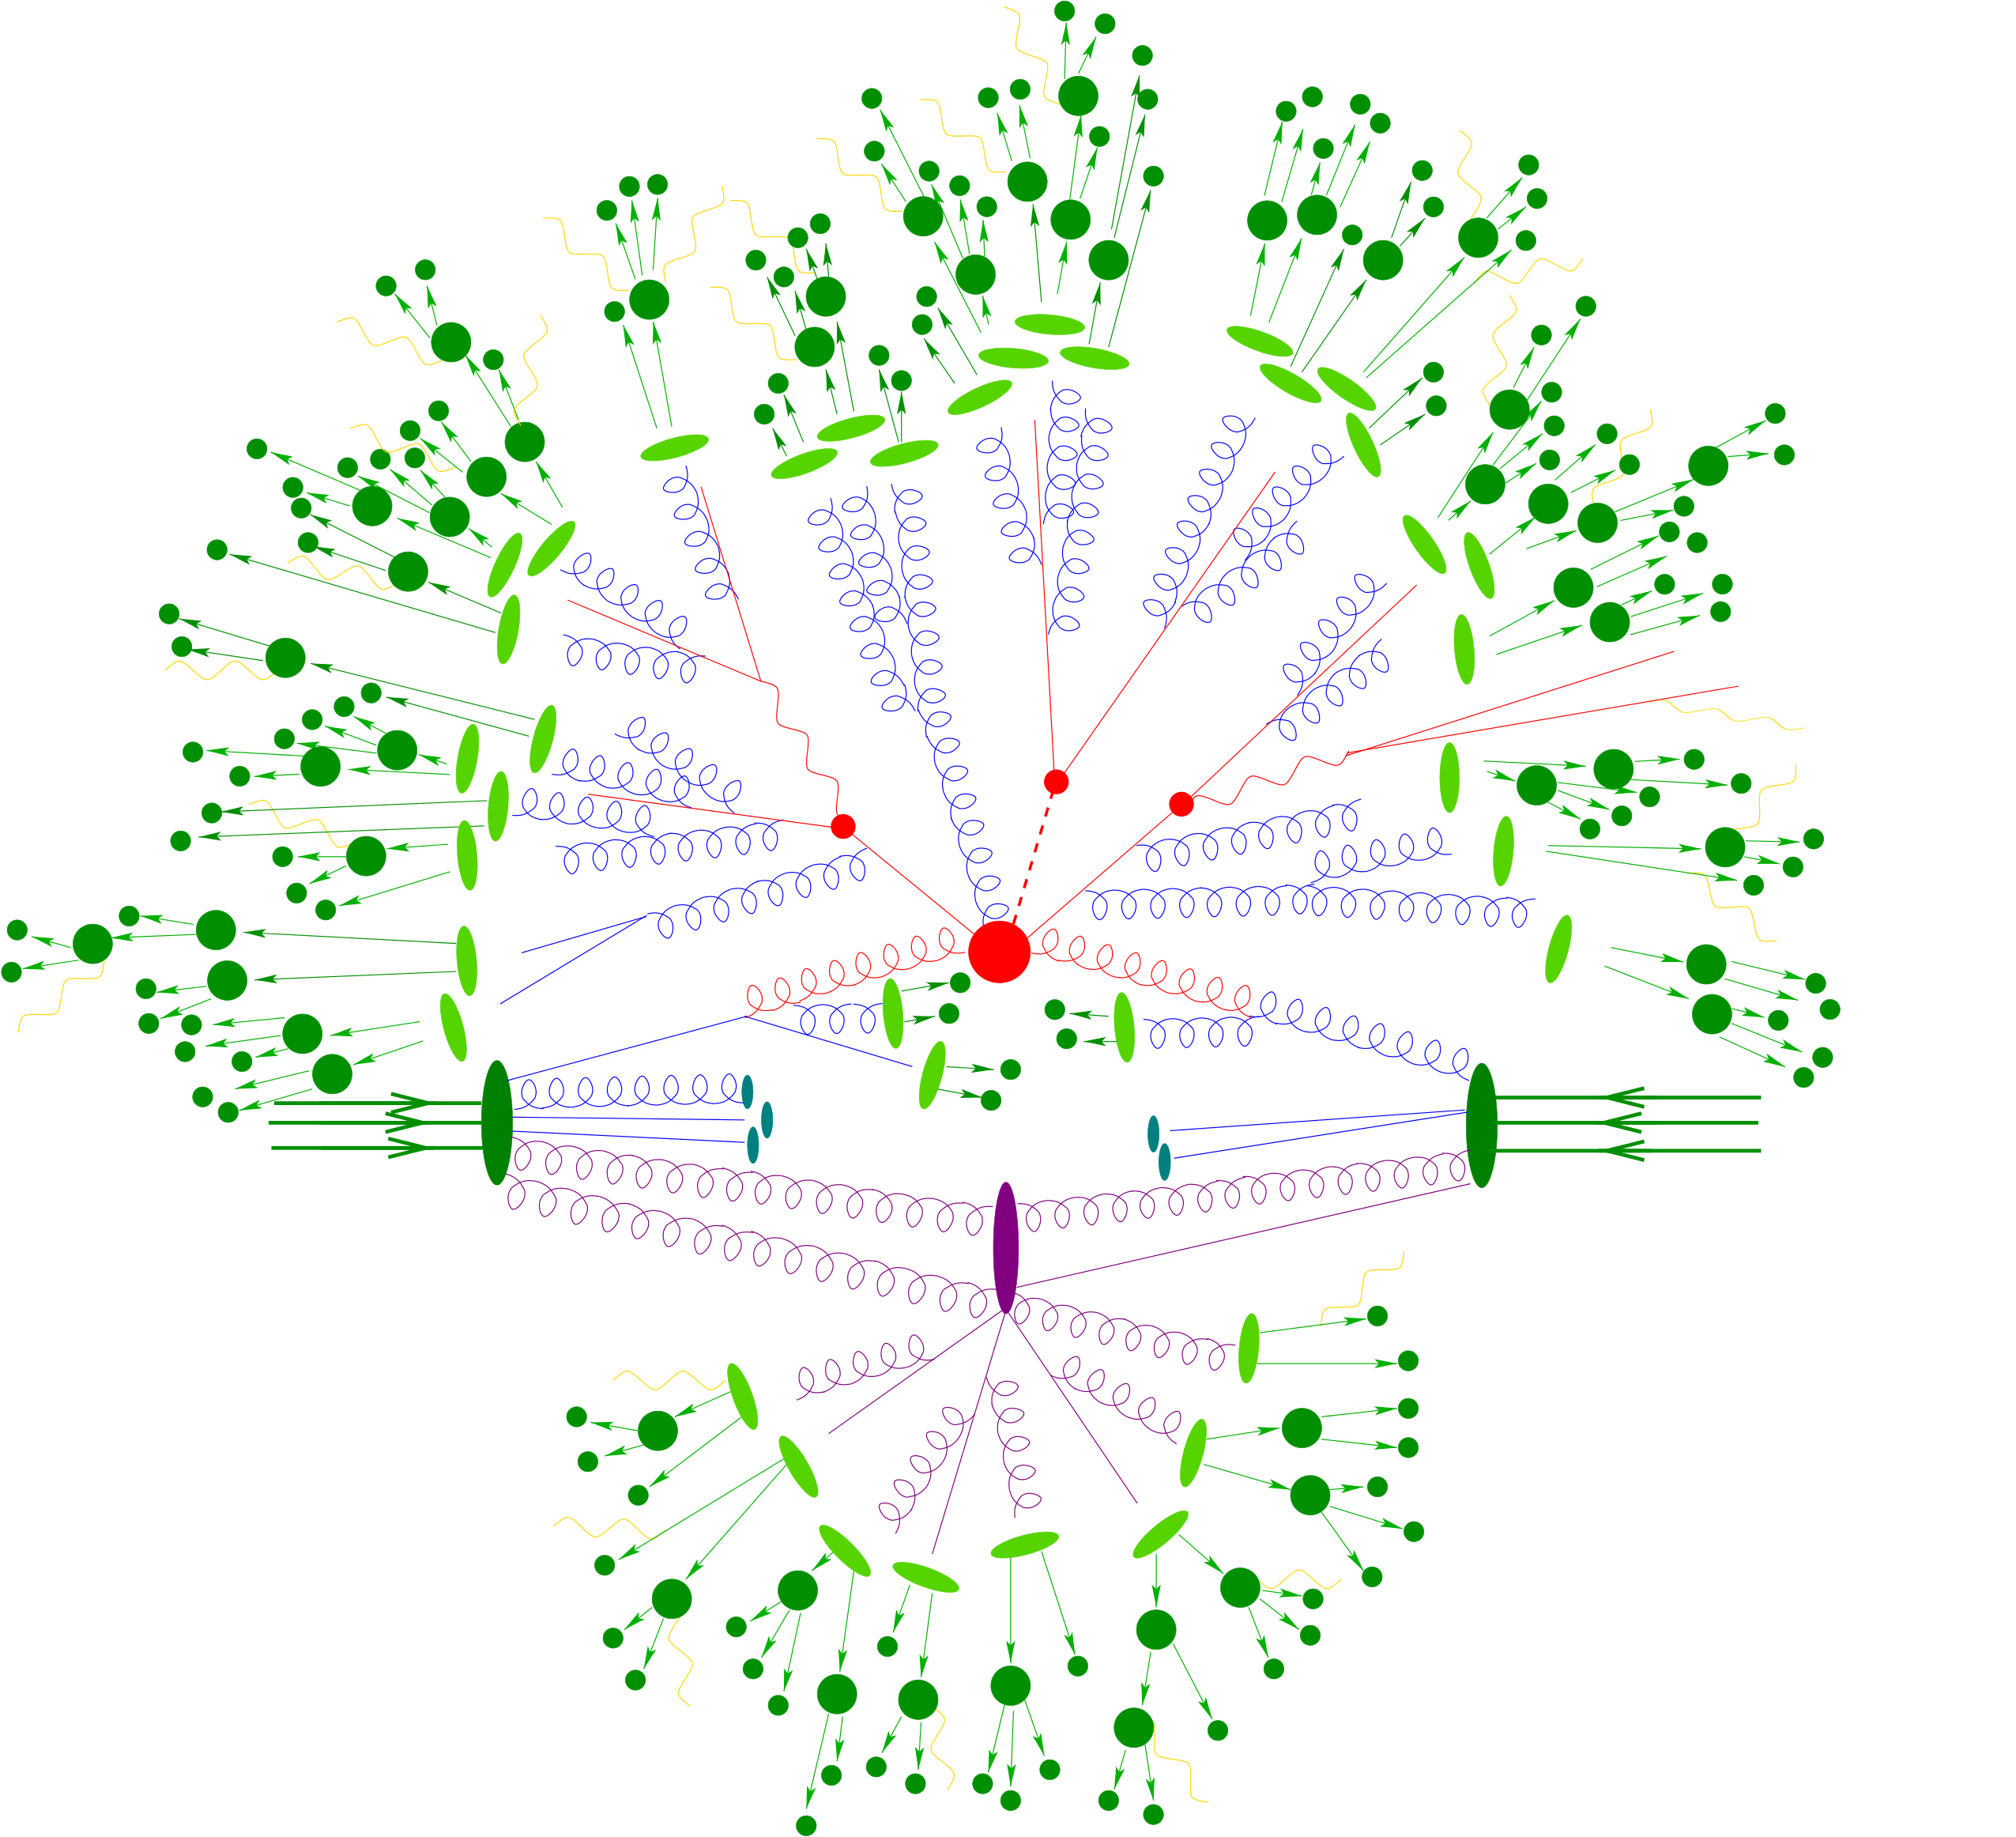
\includegraphics[width=\columnwidth]{figures/Theory/HadronEvent.jpg}
%	\caption{Simulation of a sample proton-proton collision.  The incoming partons are in blue, the underlying event interactions are in purple, the hard scattering event is in red, and the hadronization processes are shown in green.  Image from~\cite{Sherpa}.
%	}
%	\label{fig:HadronEvent}
%\end{figure}
%
%\subsection{Hard Scatter and Parton Showering}
%
%The hard scatter is the interaction of interest in an event, with two partons interacting and producing the high transverse energy final state of interest.  The Feynman diagrams for a collision correspond to the hard scatter, such as the $gg\rightarrow tth$ process shown in Figure~\ref{fig:HadronEvent}.  Here, the Higgs decays into a pair of quarks, and the two top quarks decay to $bW$, with one $W$ decaying hadronically and the other leptonically, as shown in red.  In addition, the free partons from the hard process undergo parton showering, whereby a quark or gluon can radiate a nearly-collinear gluon which carries away some portion of its momentum.  In addition, a gluon can produce a quark-antiquark pair.  This process continues until the splittings reach low enough virtuality that can no longer be described perturbatively, beyond which point confinement takes effect and the partons $hadronize$ into the colorless particles which can be observed by the detector.
%
%\subsection{Pileup and Underlying Event}
%
%The underlying event, shown in purple in Figure~\ref{fig:HadronEvent}, is the interaction of the remaining partons in the $pp$ collision which did not participate in the hard scatter.  These remnants can interact with each other and produce softer interactions which then overlay with the products from the hard scatter of interest.
%
%ATLAS produces collisions by colliding bunches with $\sim10^{11}$ protons each, and as such a variable number of collisions occur each bunch crossing.  For a typical data event taken in 2016, a single hard scatter event was also accompanied by some two dozen other softer scatters, often referred to as pileup.  The distribution of the number of pileup interactions can be seen in Figure~\ref{fig:LumiPileup}.  Pileup takes two forms: in-time pileup which produces particles which appear simultaneously in the detector with the hard scatter products, and out-of-time pileup where particles from previous bunch crossings are still traveling through the detector.
%
%The effect of both the underlying event and a single pileup event is roughly the same: it adds additional calorimeter noise and physics objects which make it more difficult to pick out only the hard scatter products.  An example event is shown in Figure~\ref{fig:PileupEvent} where a single $Z\rightarrow\mu\mu$ event with 24 pileup interactions is shown.  All of the energy deposited in the calorimeter, with the exception of the small amount along the path of the muons, comes from the underlying event and pileup interactions.  While this can have a large effect on searches using lower-momentum objects or missing transverse energy, the high-mass dijet search is relatively insensitive to their effects owing to the large discrepancy in energy scales between typical pileup interactions and the hard scatters of interest.
%
%\begin{figure}[h!]
%	\centering
%	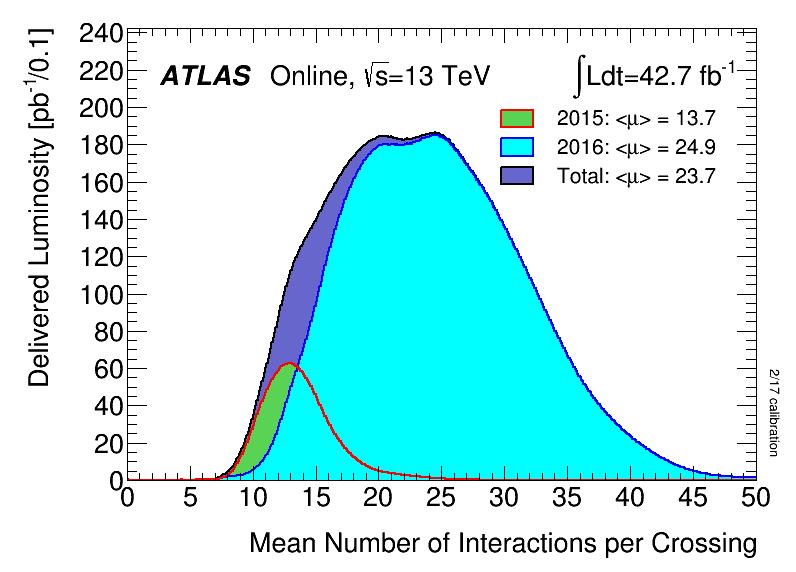
\includegraphics[width=0.5\columnwidth]{figures/Jets/LumiPileup.png}
%	\caption{Luminosity-weighted distribution of the mean number of interactions per crossing for the 2015 and 2016 datasets.
%	}
%	\label{fig:LumiPileup}
%\end{figure}
%
%\begin{figure}[h!]
%	\centering
%	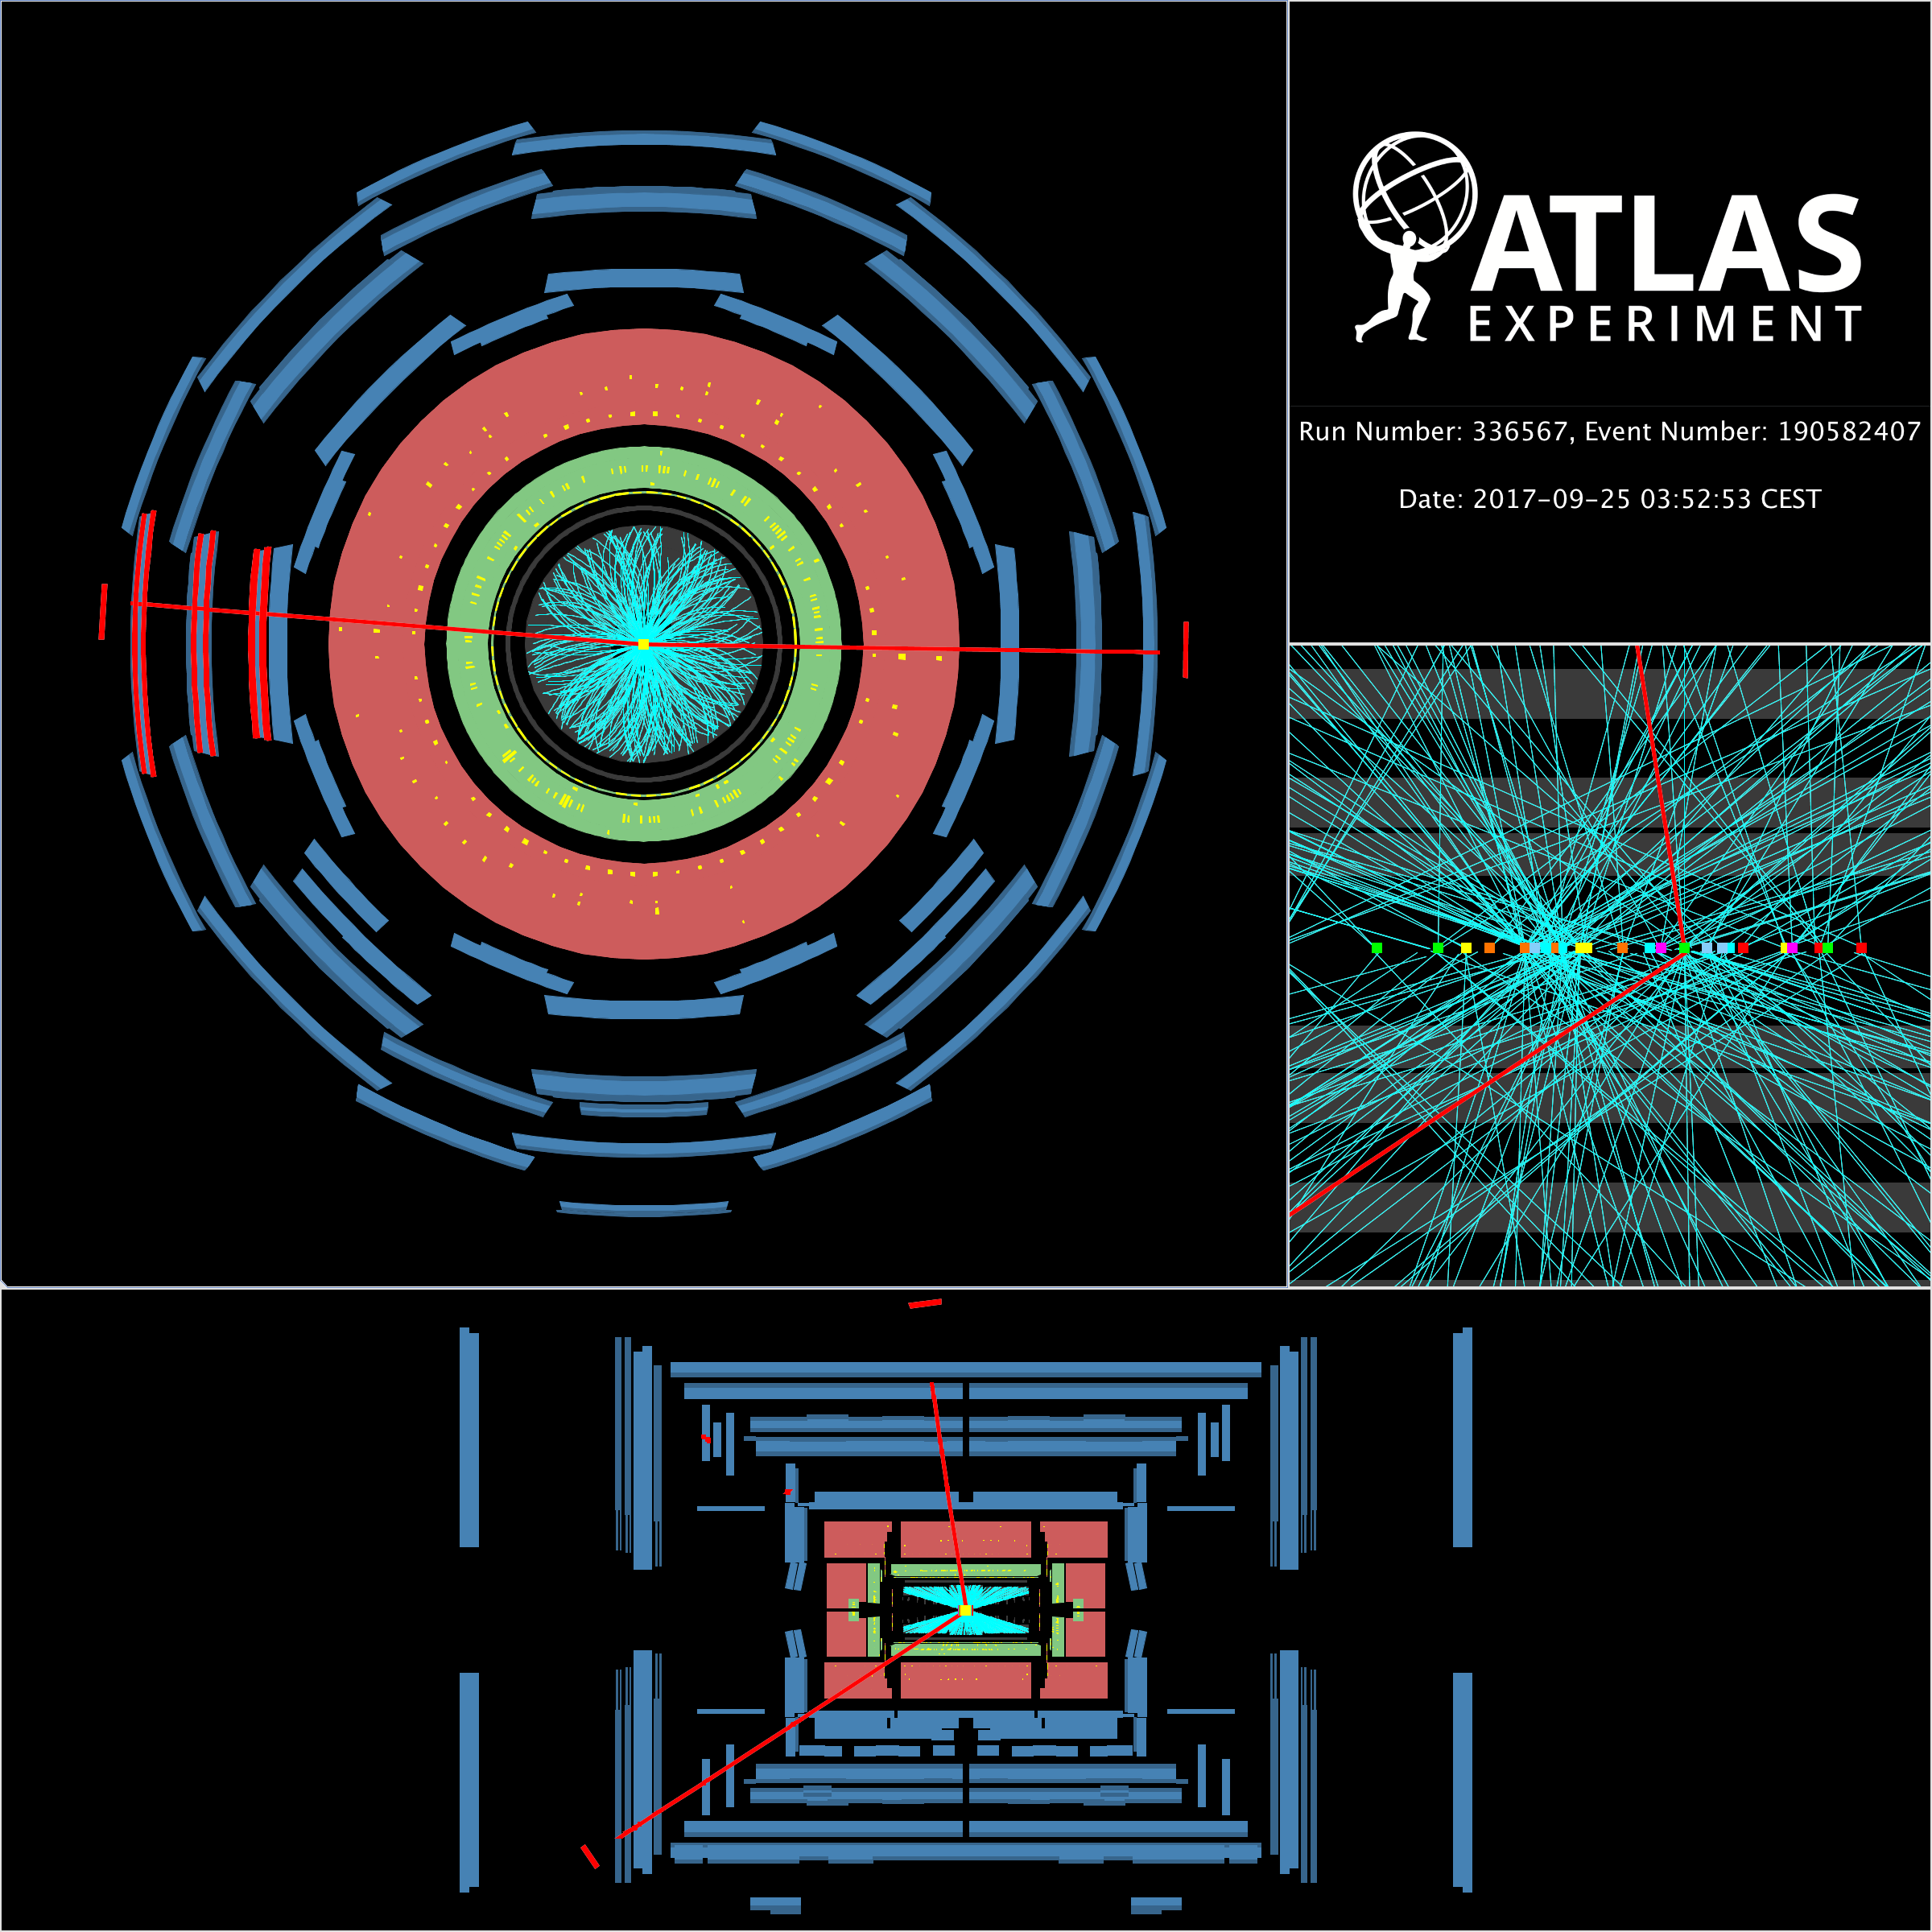
\includegraphics[width=\columnwidth]{figures/Jets/PileupEvent.png}
%	\caption{Event display of a $Z\rightarrow\mu\mu$ event with 24 other reconstructed vertices from pileup interactions.  The paths of the two muons are shown in red, while the blue lines are tracks with $\pt >$ 500\,MeV 
%	}
%	\label{fig:PileupEvent}
%\end{figure}
%
%\subsection{Hadronization}
%
%As the partons and their showering products in the collision move to longer distances, the process of hadronization occurs whereby the colored partons are formed into colorless baryons and mesons which will then decay into the final state particles which are seen by the detector.  An exact description of hadronization in QCD is not known, but there are several models used in Monte Carlo generators which work very well, including the Lund string model~\cite{LundStringModel} used in the Pythia~\cite{Pythia} generator, and the cluster model~\cite{ClusterModel} used in the Herwig~\cite{Herwig} generator.  The particular showering process used has almost no effect on the sensitivity of this analysis.
%
%\section{Jets}
%
%The partons from the hard scattering process are not experimentally observable, only the wide range of hadrons produced in the hadronization step.  However, momentum and energy are conserved throughout the showering process, and as such reflect the kinematics of the originating particle. Jets are the observable physics object for hadronic particles, roughly-conical sprays of particles which have their energies added together into a single object.
%
%The $jet$ $algorithm$ defines the method by which observables, such as the final-state particles in simulated data or calorimeter cells in a detector, are combined to create jets.  There is no one algorithm which is the correct one, and ATLAS uses several different jet definitions depending on the use case.  For example, the Level-1 jet trigger uses the very crude method of a square around a given high-energy trigger tower seed.  This is a very poor definition in general, but works very well given the constraints of the trigger.
%
%A good jet definition will be immune to small changes in the treatment of the clustered particles, often called infrared and collinear (IRC) safe.  The jet definition will return the same number of jets in both the case of an infinitesimally soft (infrared) particle being added to an event, and in the case of a hard single particle being split into two softer, collinear particles.  Some examples of the behavior of jet algorithms which are infrared or collinear unsafe are shown in Figure~\ref{fig:IRCSafety}.  IRC safety is important for linking experimental results and theoretical predictions, as these processes happen randomly through parton showering and should not change the interpretation between the original scattered particle and the jet it creates.
%
%\begin{figure}[h!]
%	\centering
%	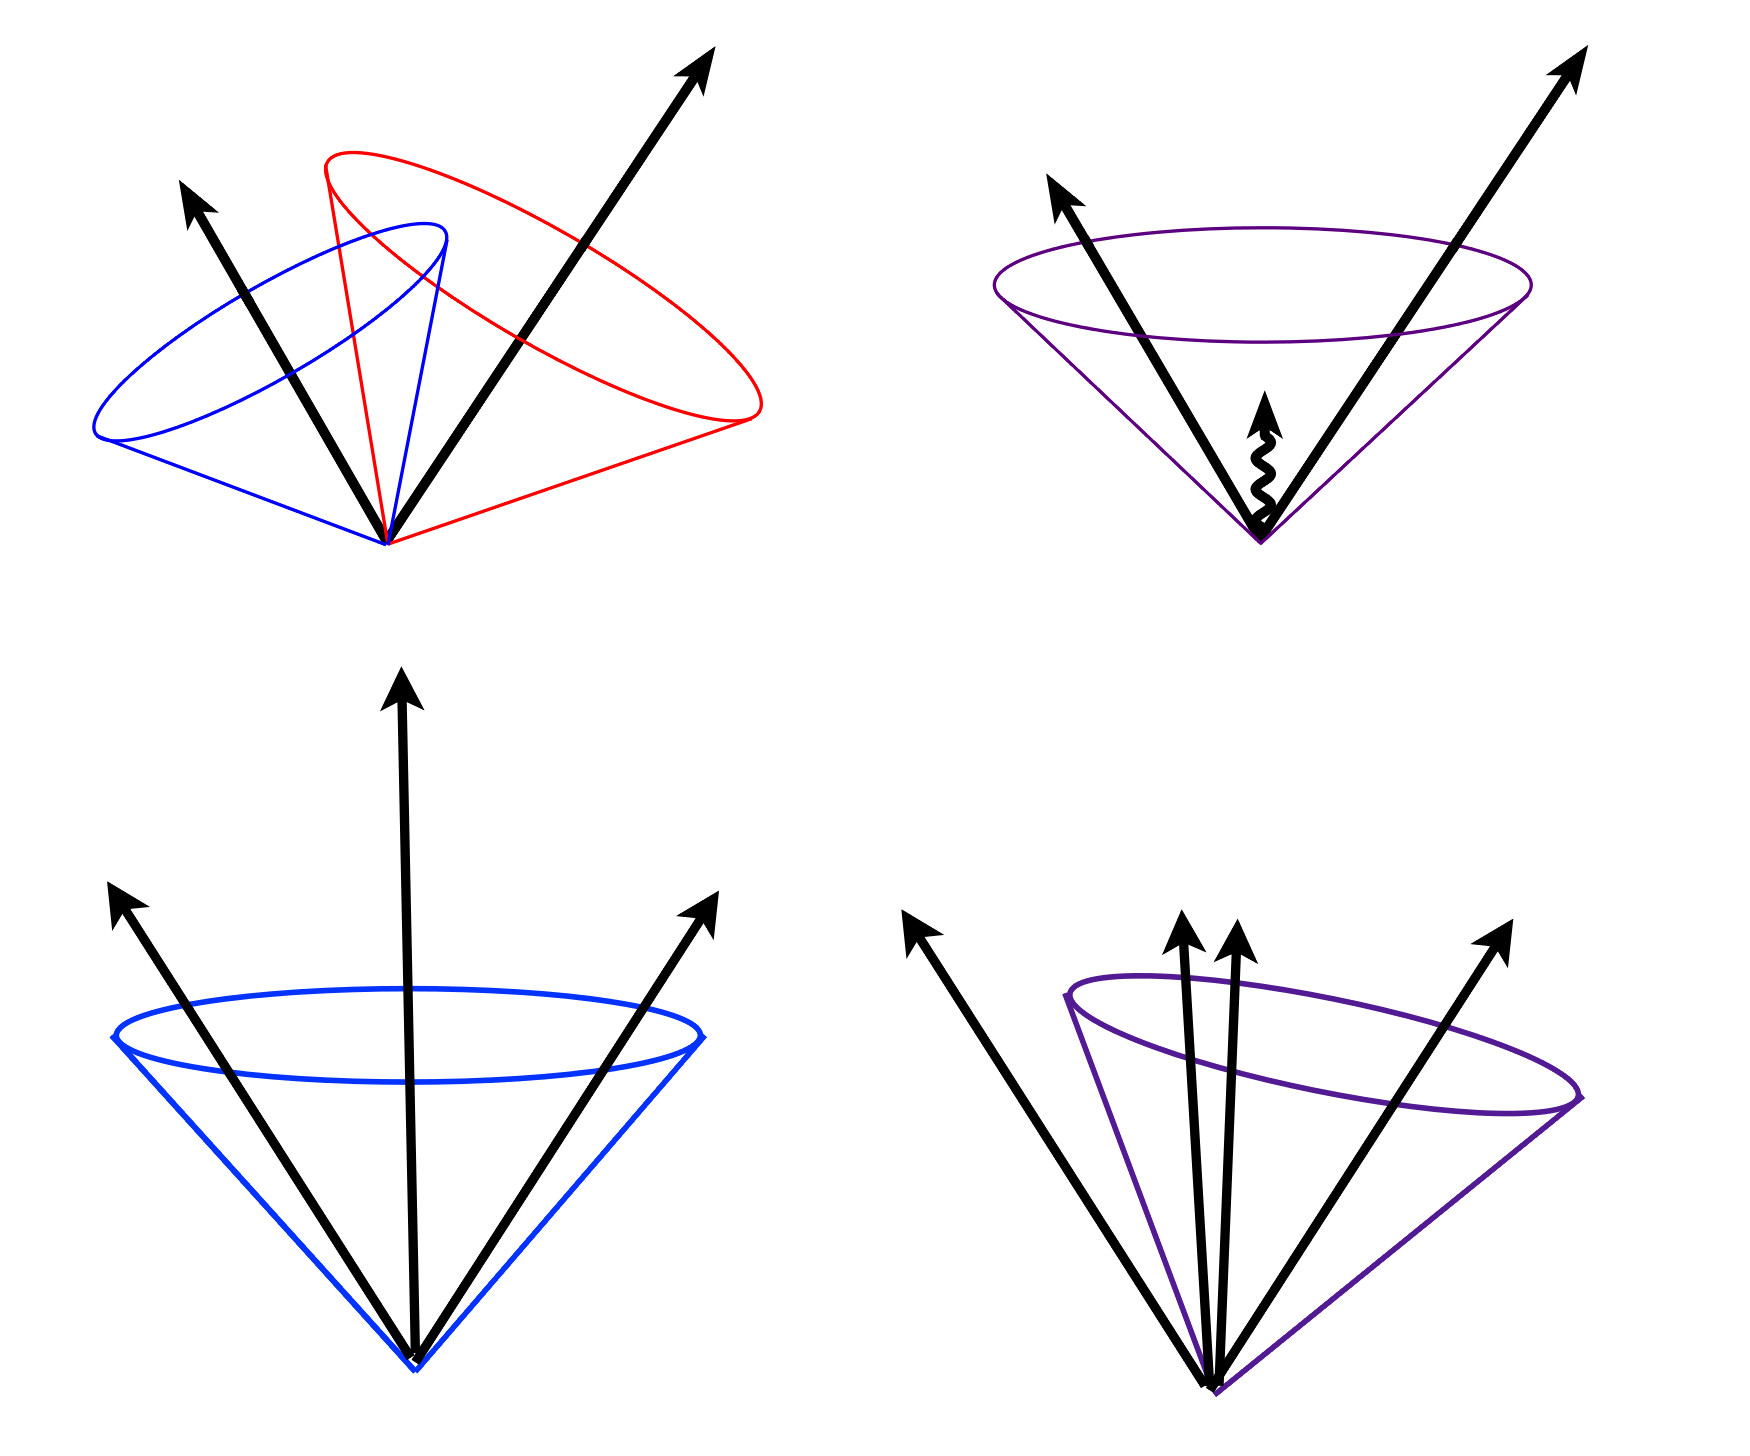
\includegraphics[width=0.7\columnwidth]{figures/Jets/IRCSafety.png}
%	\caption{Examples of the behavior of infrared and collinear unsafe jet algorithms.  In the top two diagrams, the addition of a soft gluon becomes the seed which a jet is centered on, causing the two jets to merge together into one jet.  In the bottom diagram, the splitting of the most energetic seed into two collinear ones, shifting the jet location and lowering the jet energy.  Diagram from \cite{IRCDiagram}.
%	}
%	\label{fig:IRCSafety}
%\end{figure}
%
%\subsection{The Anti-$k_t$ jet algorithm}
%A jet algorithm begins with a list of subjets, the individual inputs which will be combined to make jets.  In the case of ATLAS, the subjets are calorimeter topoclusters which are discussed in more detail in Section~\ref{sec:Topoclustering}, while for truth-level jets individual final state particles are used as subjets. The ATLAS jet definition of choice is the anti-$k_t$ algorithm.\cite{AntiKt} The anti-$k_t$ algorithm belongs to a family of sequential recombination algorithms which take the form:
%
%\begin{equation}
%	d_{ij} = \mbox{min}(k_{ti}^{2p},k_{tj}^{2p})\frac{\Delta_{ij}^2}{R^2}
%\end{equation}
%\begin{equation}
%d_{iB} = k_{ti}^{2p}
%\end{equation} 
%where $\Delta_{ij}^2 = (y_i - y_j)^2 + (\phi_i - \phi_j)^2$ is the distance between two subjets with rapidities $y_i$ and azimuths $\phi_i$, $k_{ti}$ is the transverse momentum of the subjet, and $R$ is the radius parameter which sets the size of the jet.  The parameter $p$ determines the behavior of the algorithm; $p=1$ corresponds to the $k_t$ algorithm~\cite{JetAlgos}, while $p=0$ gives the Cambridge/Aachen algorithm.\cite{CambridgeAachen}  Setting $p=-1$ gives the anti-$k_t$ algorithm.
%
%The algorithm begins by calculating $d_{iB}$ for each subjet and $d_{ij}$ for each pair of subjets, where the subjets are the input type to the algorithm.  The recombination proceeds from the smallest value of $d$.  If a $d_{ij}$ is smallest, the two subjets are combined, both their energy and their position, and all $d$ are recalculated using the new set of subjets.  If a $d_{iB}$ is smallest, the subjet is considered to be a full jet and is removed from the list of subjets.  An illustration of how this method proceeds is shown in Figure~\ref{fig:AKTExample}.
%
%\begin{figure}[]
%	\centering
%	\subfloat[]{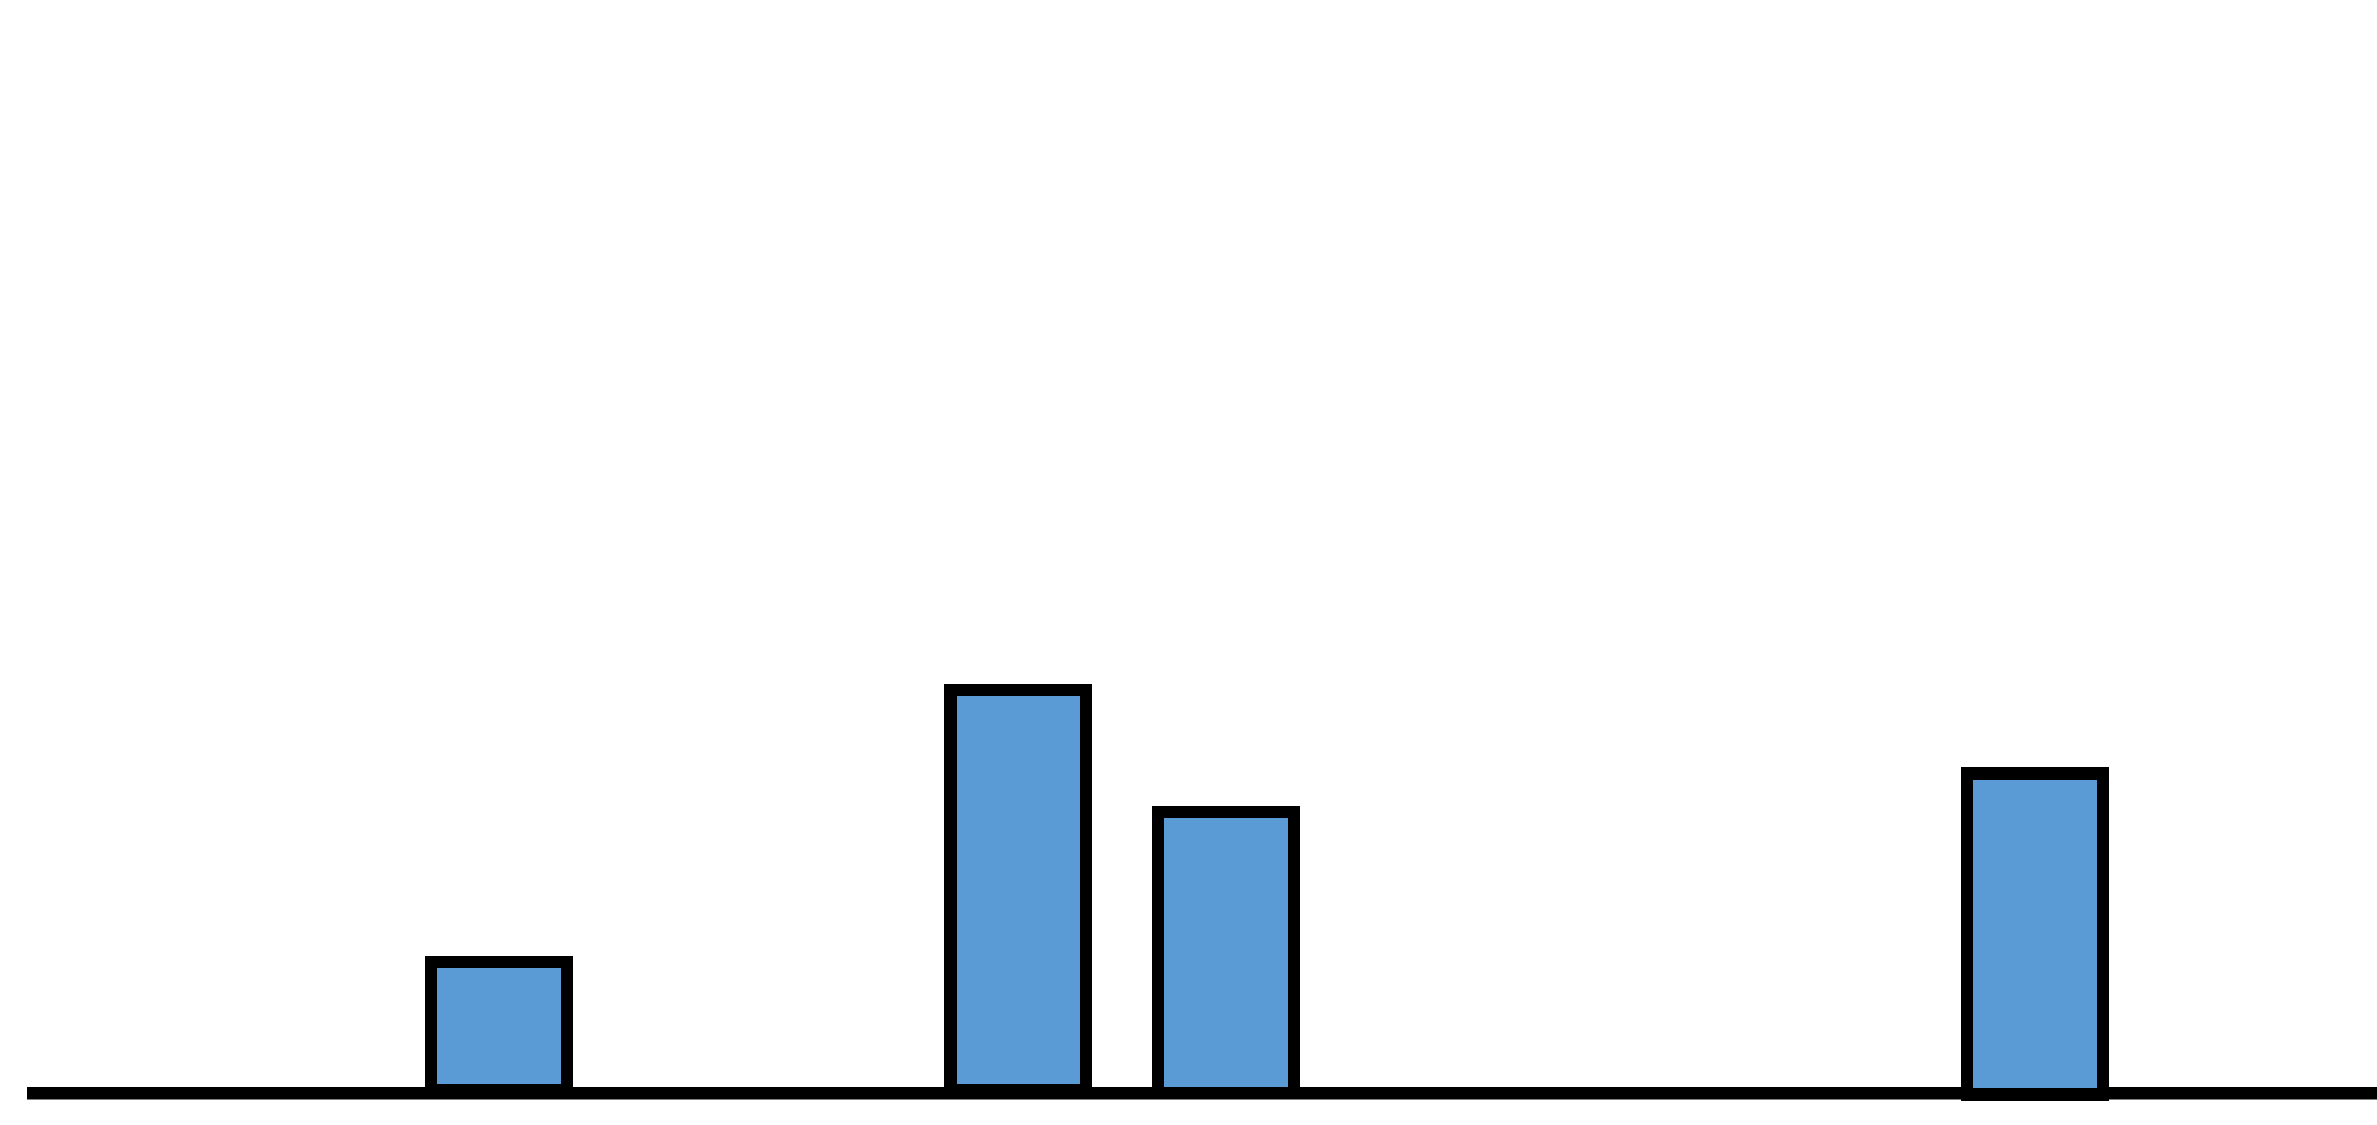
\includegraphics[width=0.45\columnwidth]{figures/Jets/AntiKt1.png}}
%	\hspace{0.1\columnwidth}%
%	\subfloat[]{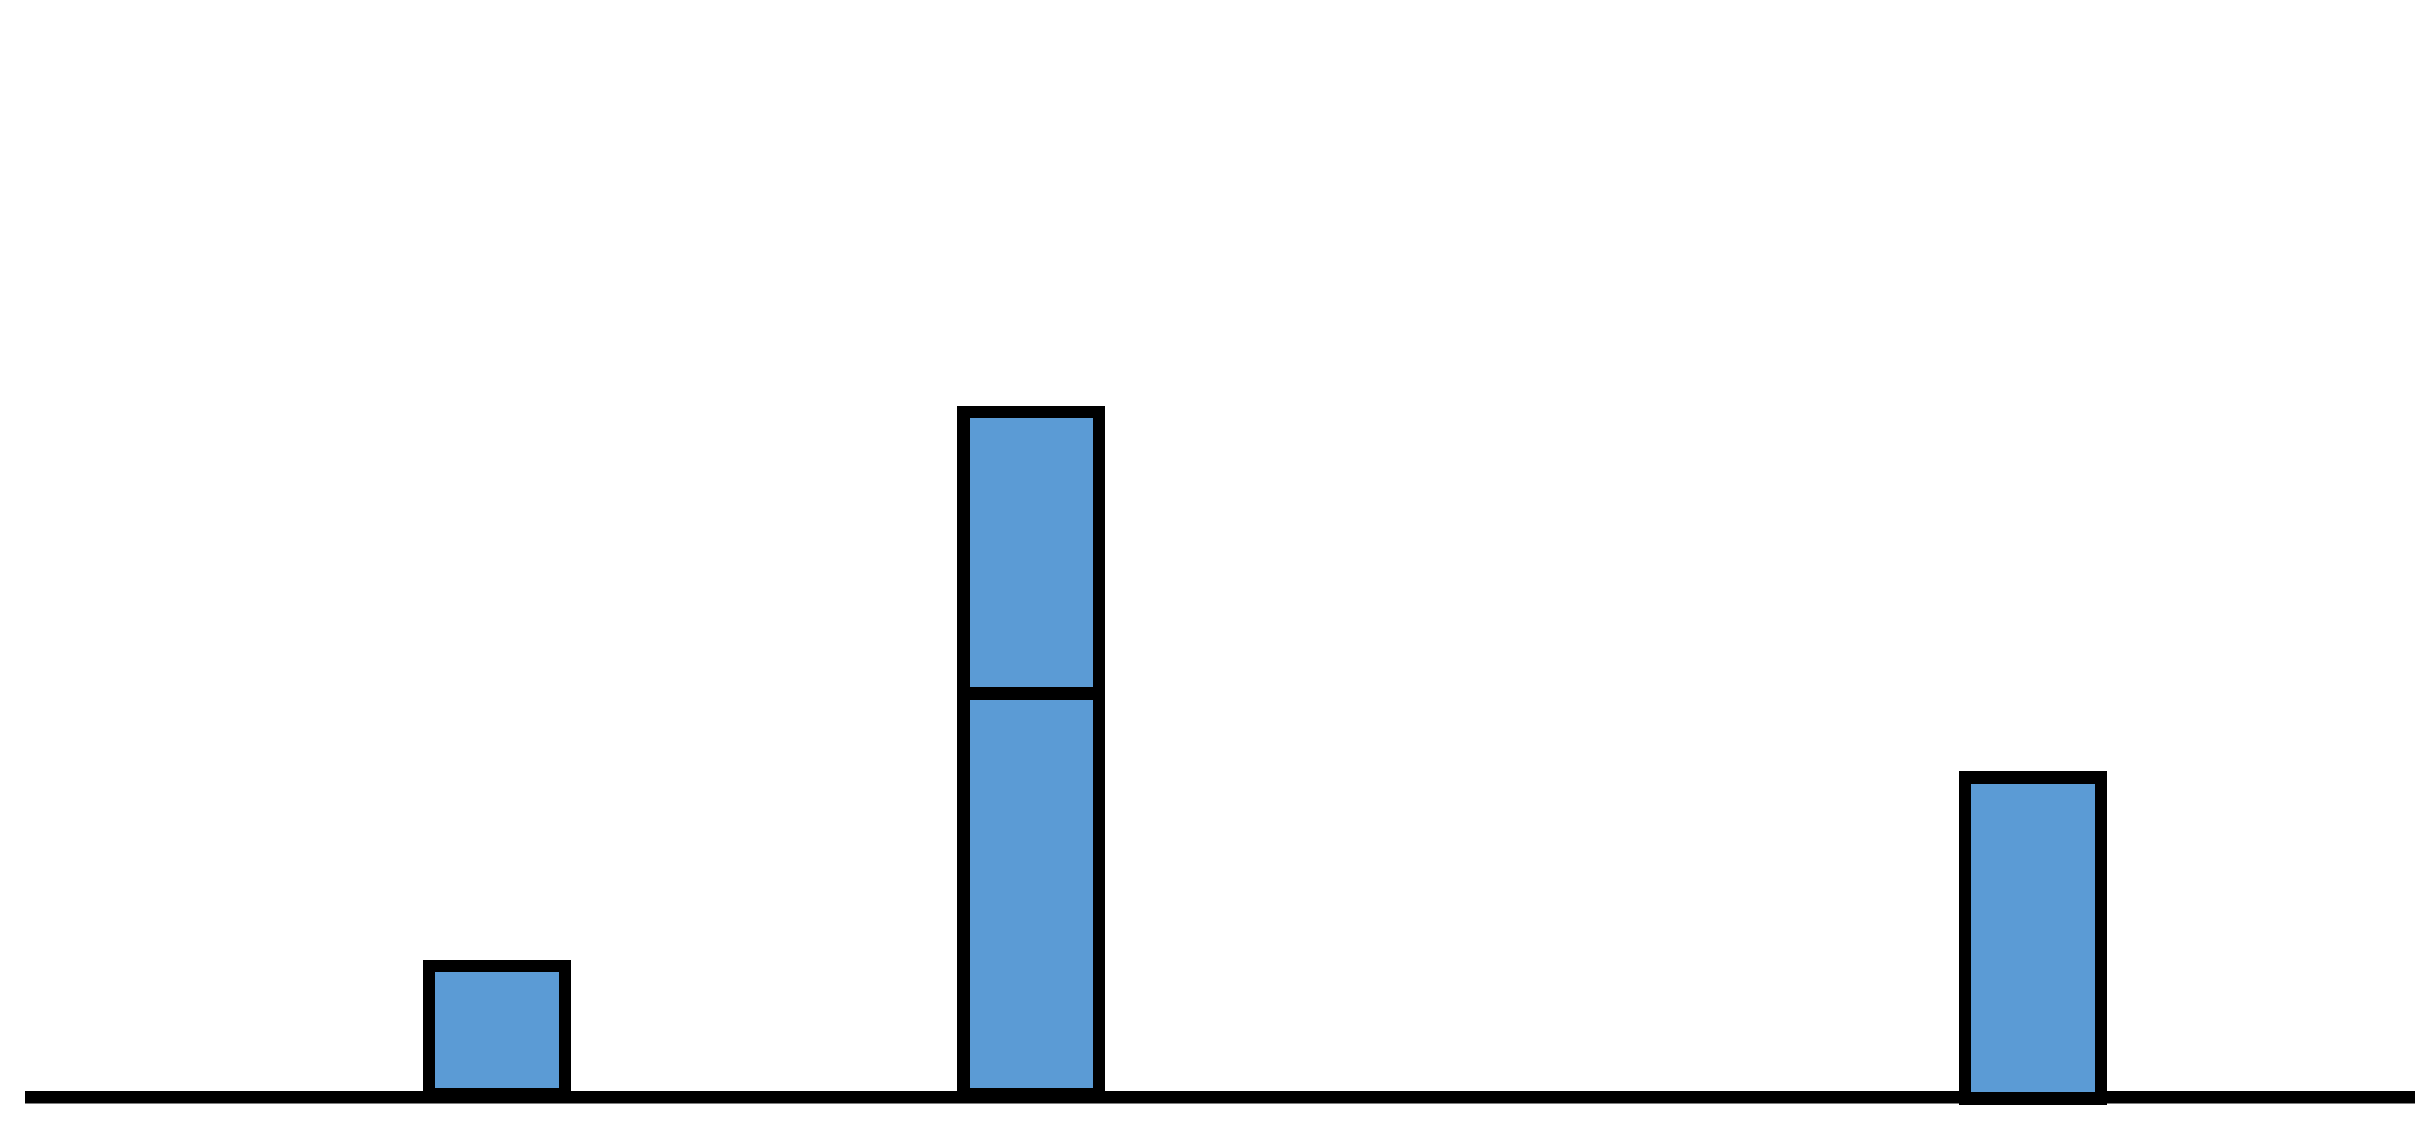
\includegraphics[width=0.45\columnwidth]{figures/Jets/AntiKt2.png}}
%	\hspace{0.1\columnwidth}%
%	\subfloat[]{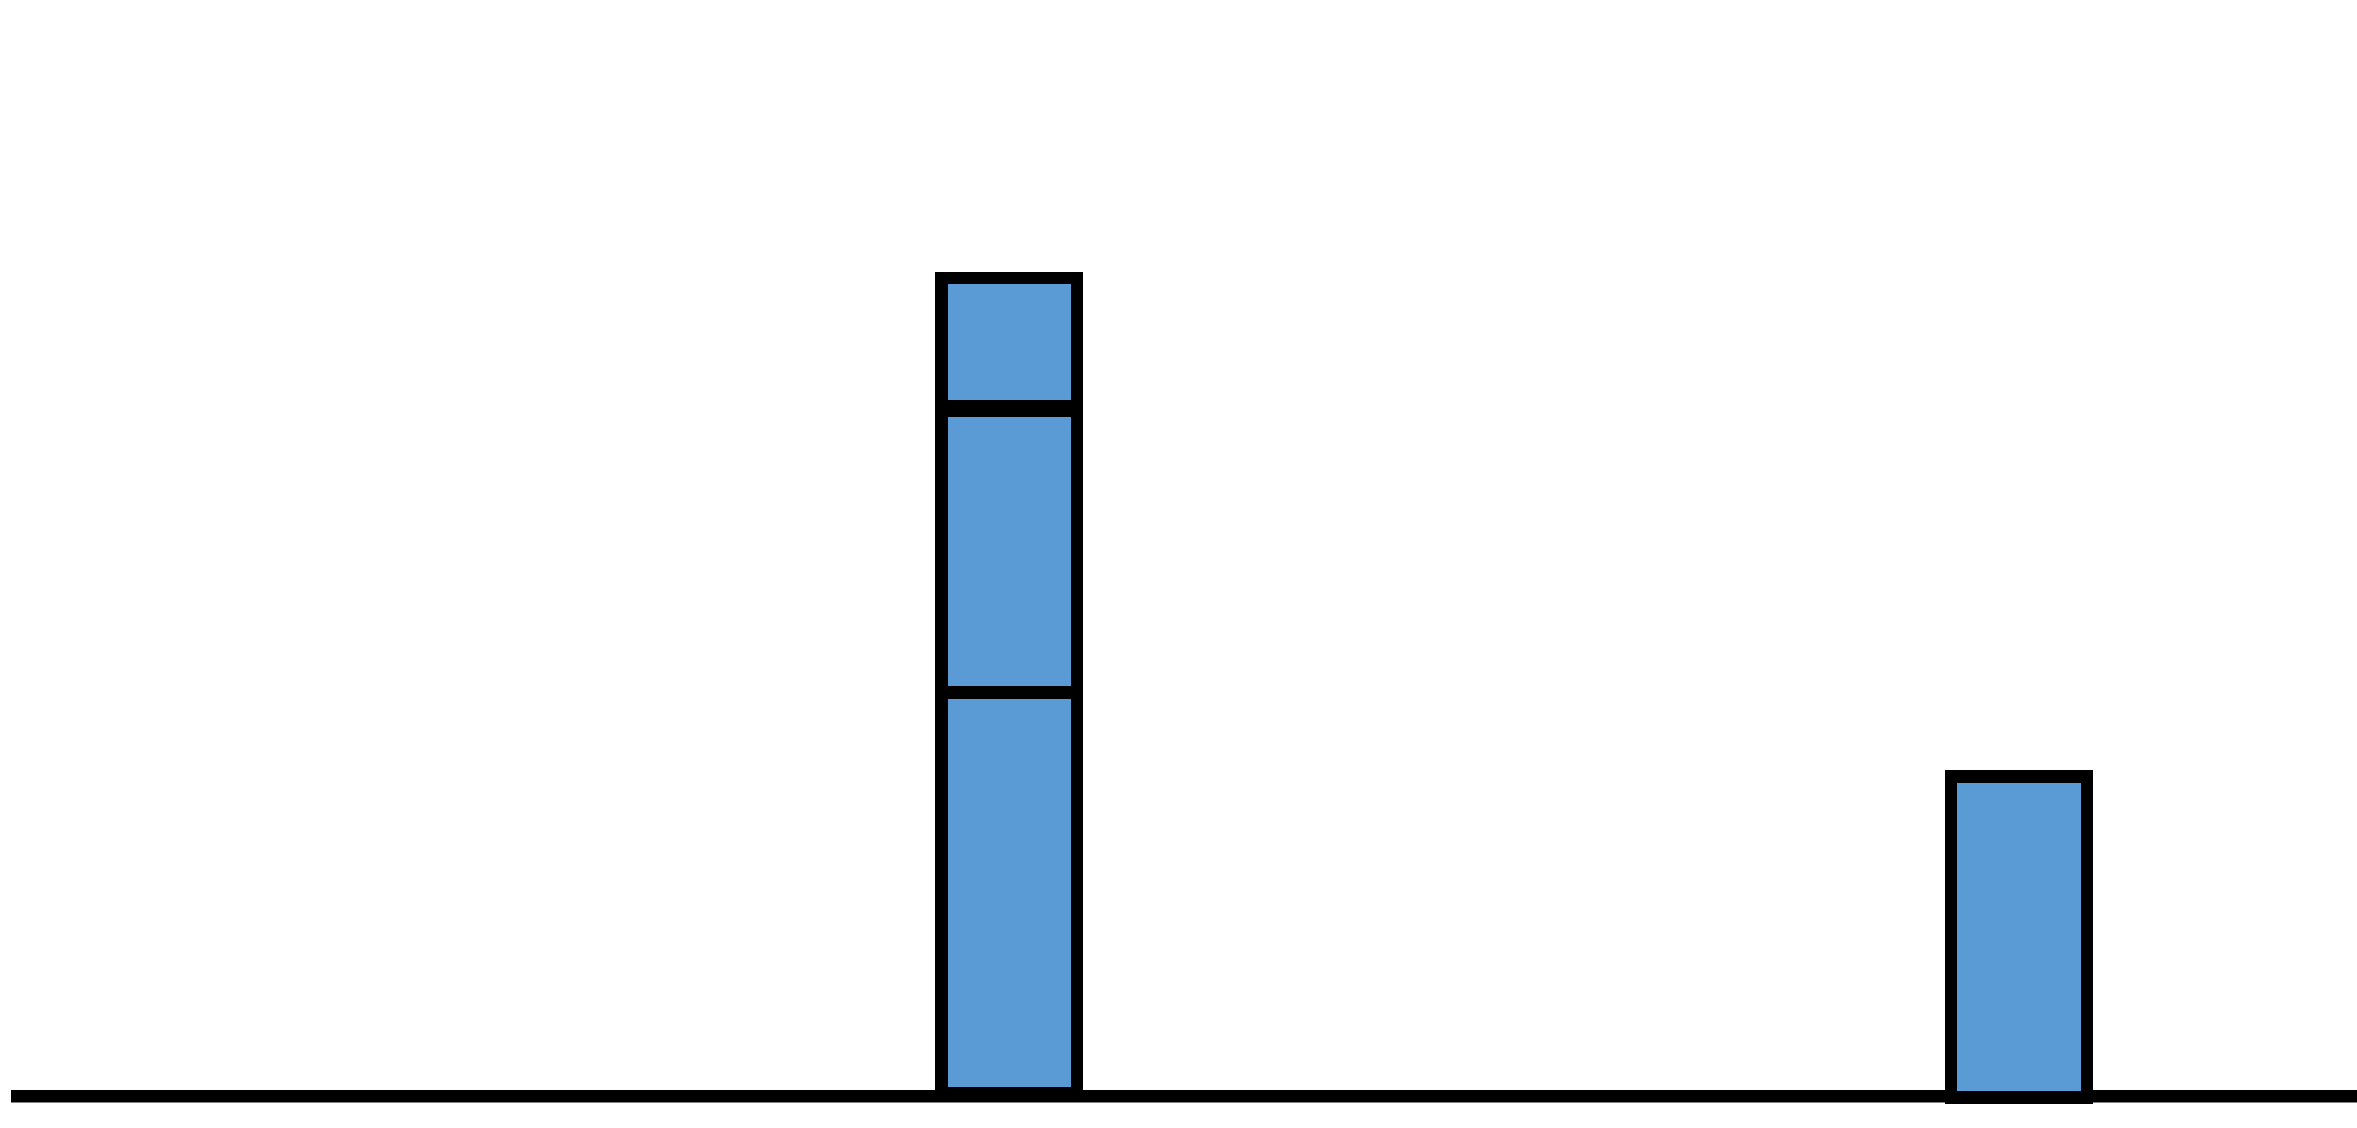
\includegraphics[width=0.45\columnwidth]{figures/Jets/AntiKt3.png}}
%	\hspace{0.1\columnwidth}%
%	\subfloat[]{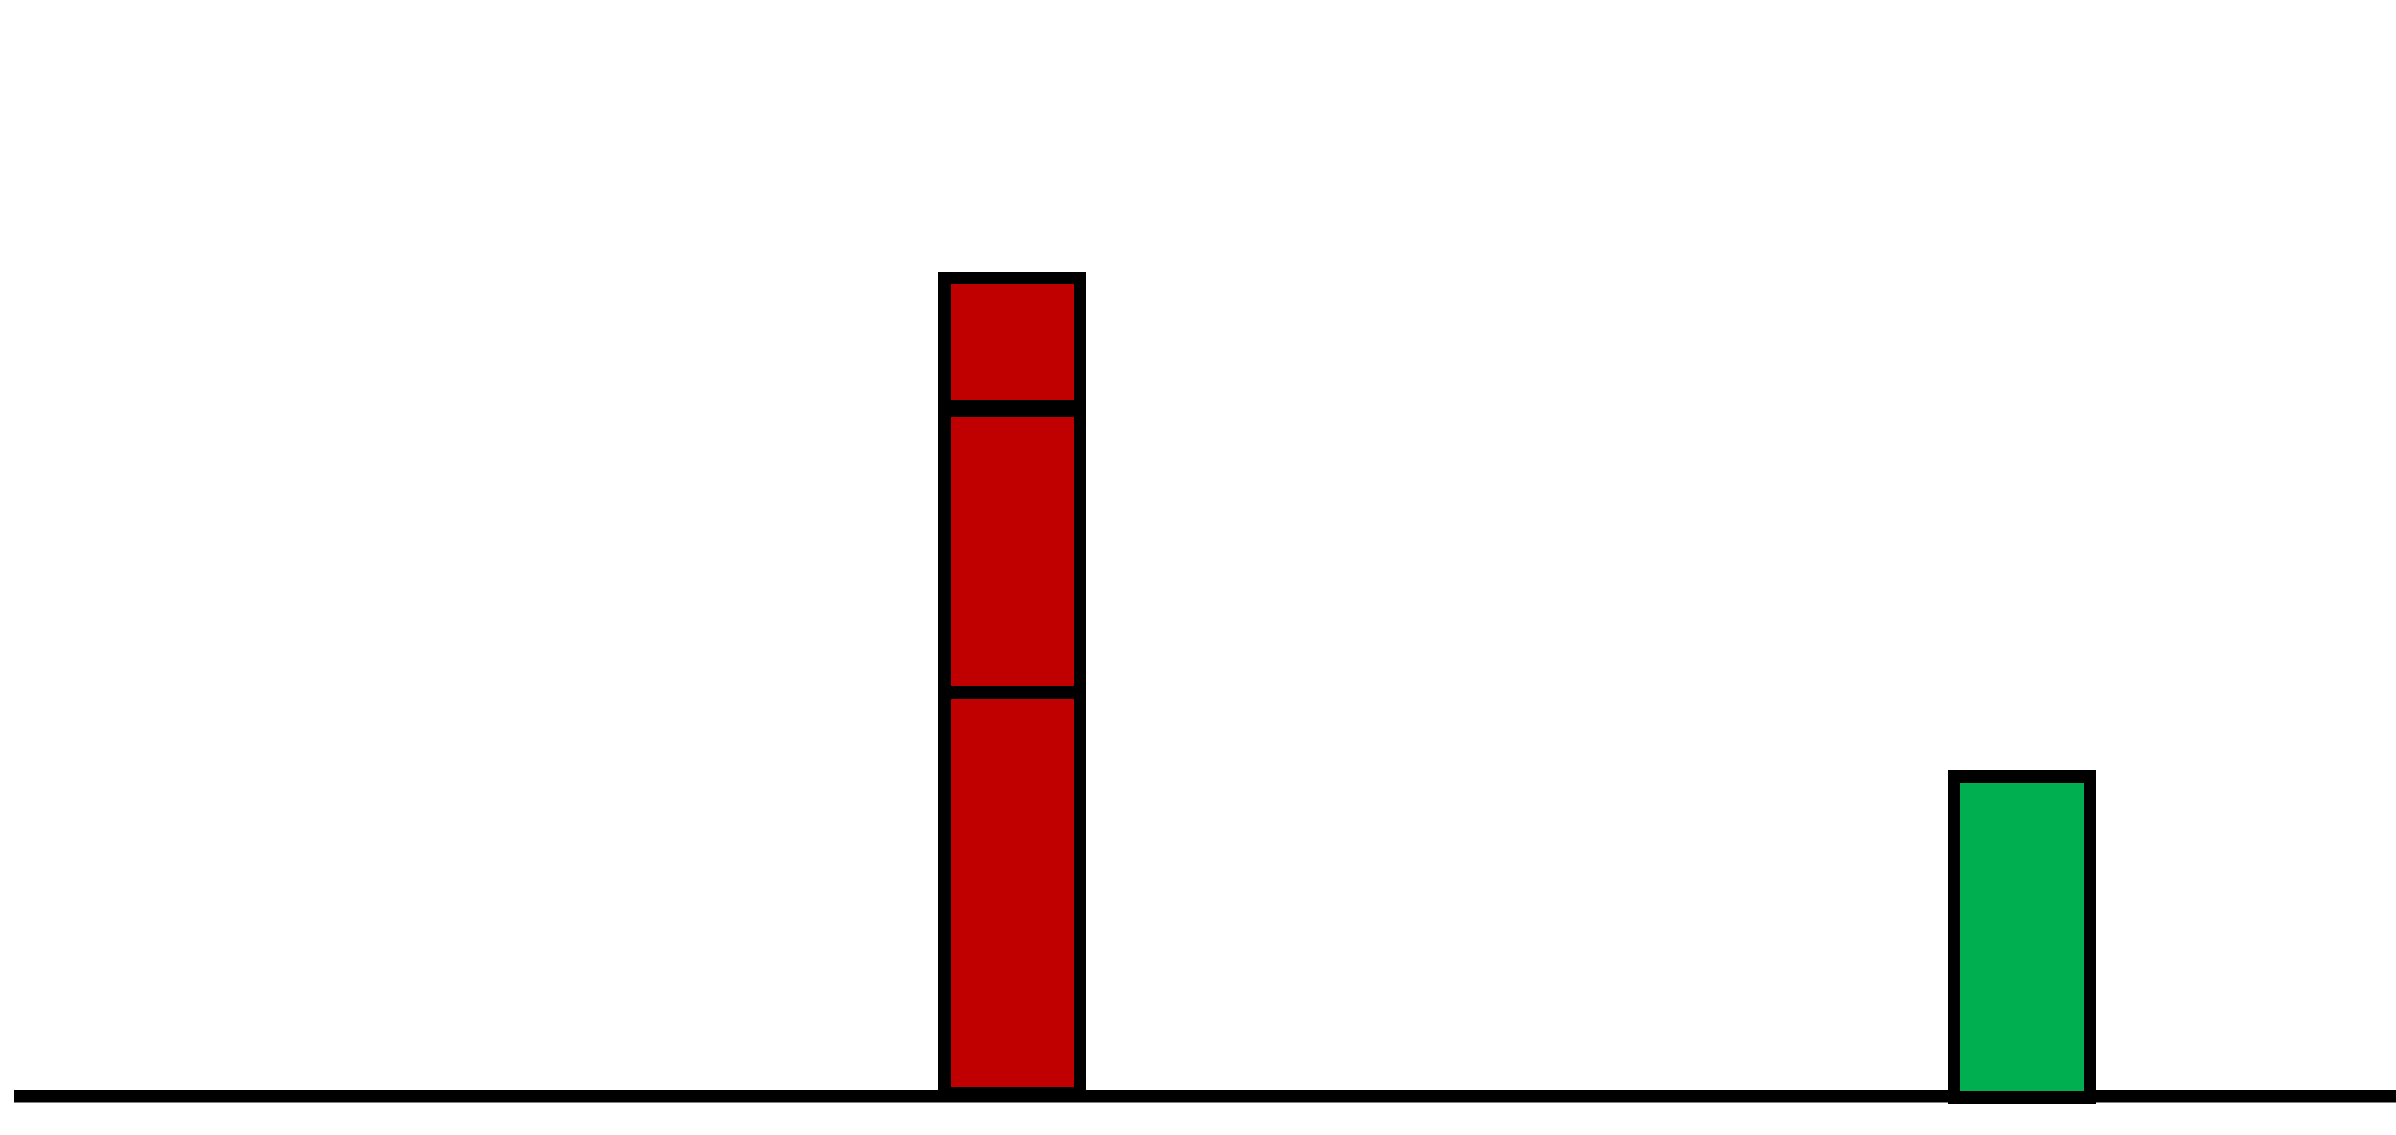
\includegraphics[width=0.45\columnwidth]{figures/Jets/AntiKt4.png}}
%	\caption{An example of the anti-$k_t$ recombination algorithm.  a) The original input subjets to the algorithm.  b) The highest \pt~subjet combines with its nearest neighbor to produce a new combined subjet.  c) This subjet again combines with its neighbor to produce a new subjet.  d) The remaining subjets are separated by more than the radius parameter of the algorithm.  The subjets become the final jets.}
%	\label{fig:AKTExample}
%\end{figure}
%
%The general behavior of the anti-$k_t$ algorithm is that the subjets with the highest transverse energy will cluster first, gathering together all of the smaller radiation around them, before the softer subjets begin clustering together.  The algorithm tends to produce roughly-conical jets, and gives preference to more energetic jets when two jets are close together.  An example of the final result of the anti-$k_t$ algorithm is shown in Figure~\ref{fig:AntiKtExample}.  Here, a single simulated event is shown along with thousands of very soft "ghost" particles which are randomly distributed and do not contribute any meaningful energy to the event.  These ghosts are used along with the real physics energy deposits in the jet algorithm but do not change the shape or location of the jets, allowing for the visualization and measure of the area encompassed by each jet.  This area is used to correct for the amount of pileup energy which falls within a jet.
%
%
%
%\begin{figure}[]
%	\centering
%	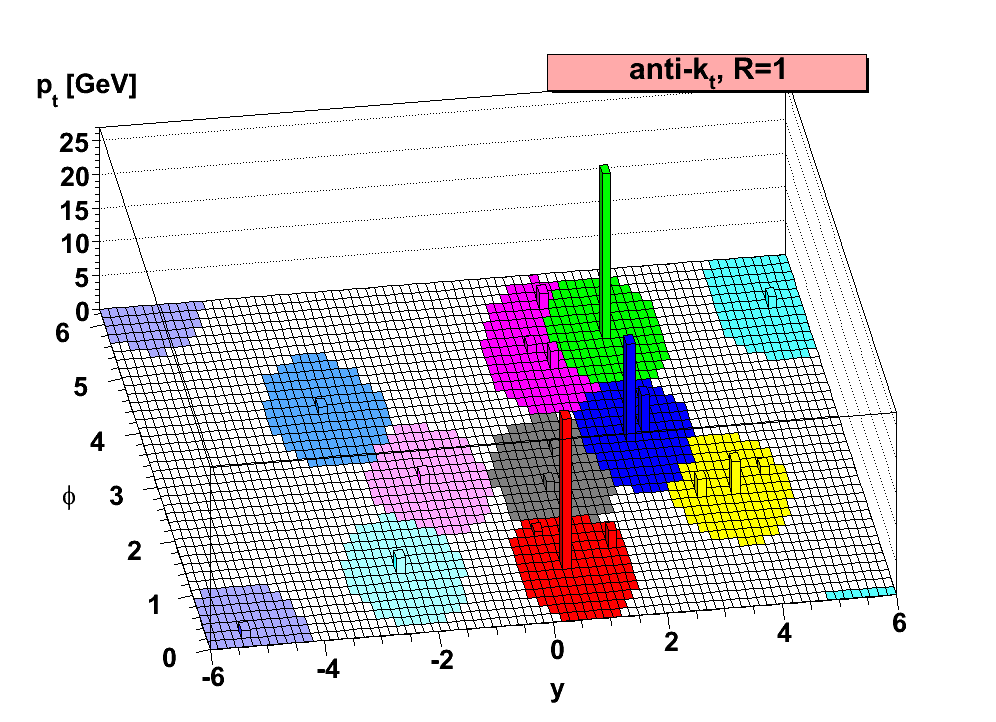
\includegraphics[width=0.7\columnwidth]{figures/Jets/AntiKtExample.png}
%	\caption{A sample parton-level event together with many random soft particles, clustered together using the anti-$k_t$ algorithm.\cite{AntiKt}.
%	}
%	\label{fig:AntiKtExample}
%\end{figure}
%
%As mentioned previously, the model of hadronization used to simulate the processes studied in this analysis has no meaningful impact on the sensitivity.  This is because the treatment of the hadronization step does not impact the location of the high-\pt~particles, but rather the distribution of soft emissions between them, and as such will have little impact on the \pt~as measured by the jet algorithm.
%
%The anti-$k_t$ algorithm is both collinear and infrared safe.  In the case of a collinear splitting of a hard particle into two softer ones, their small angular separation $\Delta_{ij}$ ensures that they will be clustered together at the beginning of the recombination, recovering the single hard particle.  The algorithm is infrared safe because a soft emission will first cluster to a highly energetic one and will not shift the jet, preventing any change in the final jet.  The choice of jet radius is somewhat arbitrary and depends on the physics process being investigated.  The standard ATLAS jet uses R=0.4, but other radii are used in specialized contexts such as R=0.2 jets to investigate jet substructure, and R=1.0 jets to capture the energy of boosted objects such a top quarks. 
